% !TEX program = lualatex
\documentclass[12pt,a4paper]{article}
\usepackage[T1]{fontenc}
\usepackage[utf8]{inputenc}
\usepackage{lmodern}
\usepackage{geometry}
\geometry{margin=1in}
\usepackage{setspace}
\usepackage{microtype}
\usepackage{amsmath,amssymb,bm}
\usepackage{booktabs}
\usepackage{enumitem}
\usepackage{hyperref}
\usepackage[authoryear,round,semicolon]{natbib}

\setlength{\parskip}{0.6em}
\setlength{\parindent}{0pt}
\onehalfspacing
\setcitestyle{aysep={,},round,semicolon}

\title{\textbf{A Typology of Theoretical Failure: How Mathematical Formalism Decouples from Physical Meaning}}
\author{}
\date{}

\begin{document}

\maketitle

% ==========================================================
\section*{Abstract}
% ==========================================================
This essay develops a diagnostic framework for evaluating theoretical rigor across physics, cognitive science, and artificial intelligence. By comparing three case studies—CIITR (Comprehension as Thermodynamic Persistence), Nikolaou et al.’s injectivity theorem for language models, and the Relativistic Scalar–Vector Plenum (RSVP) framework—it constructs a typology of theoretical failure, identifying eight recurrent breakdowns through which mathematics detaches from physical meaning. These range from dimensional incoherence and definitional circularity to mapping ambiguity and the elegance fallacy. Using the geometry of semantic manifolds, the essay recasts “understanding” as the maintenance of non-singular, energy-coupled mappings between conceptual spaces. Rigor becomes an energetic property: the ability to sustain phase-coherent correspondence between formalism and reality with finite work. The resulting diagnostic matrix translates epistemic virtues—operational definition, mathematical consistency, empirical accessibility, and cross-domain mapping—into measurable constraints on theoretical practice. Where information flow remains injective, empirically coupled, and energetically efficient, meaning endures; where it breaks, theory dissolves into rhetoric.

% ==========================================================
\section*{0. Mathematical Preliminaries: The Geometry and Thermodynamics of Meaning}
% ==========================================================

The following mathematical preliminaries formalize the geometric and thermodynamic quantities that appear throughout this paper. They introduce the minimal structure required to treat ``meaning'' as a measurable coupling between theory and reality, linking information geometry \citep{jaynes1957information} and the thermodynamics of computation \citep{landauer1961irreversibility,bennett1982thermodynamics} to the statistical mechanics of complex systems \citep{sethna2006statistical,bianconi2025entropy}.

\subsection*{0.1 Conceptual Manifolds}

Each \emph{theory} $\mathcal{T}$ is modeled as a smooth manifold $M_\mathcal{T}$ with coordinates $x^i$ representing its primitive variables (e.g., energy, entropy, curvature, or activation values). Each \emph{phenomenal domain} $\mathcal{R}$ (physical reality, data, experiment) is another manifold $M_\mathcal{R}$ with coordinates $y^a$ denoting measurable observables. A theory’s explanatory mapping is a differentiable map
\[
f : M_\mathcal{R} \to M_\mathcal{T}, \qquad y^a \mapsto x^i = f^i(y^a),
\]
whose inverse $f^{-1}$, when it exists, gives prediction or reconstruction.

\subsection*{0.2 Injectivity, Surjectivity, and Semantic Stability}

The Jacobian
\[
J^i_{\ ;a} = \frac{\partial f^i}{\partial y^a}
\]
encodes the local semantic structure of the theory. Following the information-preservation logic of \citet{nikolaou2025injective}, injective regions ($\det(J^\top J)>0$) preserve distinct meanings, while degenerate regions ($\det(J^\top J)=0$) collapse different physical situations to identical symbols. Surjectivity, $\mathrm{rank}(J)=\dim M_\mathcal{R}$, ensures the theory spans all empirical possibilities.

\subsection*{0.3 Phase Coherence and Energetic Coupling}

To model the energetic maintenance of correspondence, assign each mapping an instantaneous phase difference
\[
\phi(y,t)=\theta_\mathcal{T}(y,t)-\theta_\mathcal{R}(y,t),
\]
where $\theta_\mathcal{T}$ and $\theta_\mathcal{R}$ represent the phases of theoretical and empirical oscillations. The mean alignment power,
\[
P=\frac{1}{V}\int_{M_\mathcal{R}}\cos^2[\phi(y,t)]\,dV,
\]
serves as a dimensionless measure of semantic coherence analogous to synchronization metrics in nonequilibrium thermodynamics \citep{bianconi2025entropy}.

\subsection*{0.4 Work of Understanding}

Maintaining low phase error requires energy. Let $E(t)$ be the cumulative work needed to minimize phase drift:
\[
E(t)=\int_0^t \gamma\,|\dot{\phi}|^2\,dt',
\]
where $\gamma$ is a coupling constant representing interpretive resistance. This defines the \emph{Work of Understanding},
\[
W=\gamma\int|\nabla\phi|^2\,dV,
\]
analogous to the energy of a spin field maintaining orientation under dissipative forcing \citep{sethna2006statistical}.

\subsection*{0.5 Entropic Cost and Information Conservation}

If $S_\mathcal{T}$ and $S_\mathcal{R}$ are entropy measures over theoretical and empirical distributions, the entropy gap $\Delta S=S_\mathcal{T}-S_\mathcal{R}$ quantifies interpretive dissipation. By Landauer’s bound \citep{landauer1961irreversibility}, the energetic cost of comprehension satisfies
\[
W \ge k_B T\,\Delta S.
\]
This connects meaning maintenance directly to physical resource expenditure \citep{bennett1982thermodynamics}.

\subsection*{0.6 Summary of Key Relations}

\begin{table}[htbp]
\centering
\begin{tabular}{lll}
\toprule
Concept & Symbolic condition & Interpretation \\
\midrule
Injectivity & $\det(J^\top J)>0$ & No loss of meaning \\
Surjectivity & $\mathrm{rank}(J)=\dim M_\mathcal{R}$ & Coverage of phenomena \\
Phase coherence & $P\approx1$ & Sustained empirical coupling \\
Work of understanding & $W=\gamma\int|\nabla\phi|^2\,dV$ & Energy cost of alignment \\
Entropy balance & $W\ge k_BT\Delta S$ & Thermodynamic constraint on comprehension \\
\bottomrule
\end{tabular}
\caption{Summary of key geometric and thermodynamic relations.}
\end{table}

\subsection*{0.7 From Mathematics to Diagnosis}

Each failure mode identified later corresponds to the breakdown of one or more of these relations: dimensional incoherence $\leftrightarrow$ undefined $J$; definitional circularity $\leftrightarrow$ $\mathrm{rank}(J)=0$; empirical inaccessibility $\leftrightarrow$ undefined $M_\mathcal{R}$; mapping ambiguity $\leftrightarrow$ $\det J$ undefined; syntactic overloading $\leftrightarrow$ multiple incompatible $J$ mappings; premature unification $\leftrightarrow$ $\mathrm{rank}(J) < \dim M_\mathcal{R}$; scope inflation $\leftrightarrow$ $M_\mathcal{T}$ includes unmapped regions; phase drift $\leftrightarrow$ $P\ll1$ \citep{popper1959logic,lakatos1978methodology,hossenfelder2018lost}.

\subsection*{0.8 Epistemic Energy Functional}

All criteria can be condensed into an \emph{epistemic energy functional}
\[
\mathcal{R}[f,\phi]
= \alpha\,\det(J^\top J)
- \beta\,|\nabla\phi|^2
- \gamma\,\Delta S ,
\]
where $\alpha,\beta,\gamma>0$ weight structural, energetic, and entropic coherence. A theory that maximizes $\mathcal{R}$ maintains the strongest coupling between mathematics and reality, realizing the low-entropy ideal of scientific rigor envisioned by \citet{popper1959logic} and elaborated through thermodynamic information principles \citep{jaynes1957information,landauer1961irreversibility}.

% ==========================================================
\section{Introduction — The Persuasiveness Problem}
% ==========================================================

\subsection{The crisis of comprehension in modern theory}

The contemporary sciences face a paradox of apparent sophistication and deep confusion. Across physics, artificial intelligence, and consciousness studies, increasingly elaborate mathematical frameworks coexist with declining agreement about what their symbols denote. Grand unified theories, once the lodestar of twentieth-century physics, now proliferate as speculative architectures largely decoupled from empirical verification \citep{hossenfelder2018lost}. The same dynamic repeats in cognitive modeling and machine learning: transformer architectures achieve predictive success while remaining interpretively opaque. In both cases, formal consistency substitutes for explanatory clarity. The resulting ``crisis of comprehension'' is not a shortage of mathematics but an erosion of the energetic coupling between mathematical representation and measurable world.

Karl Popper framed scientific progress as a process of conjecture and refutation \citep{popper1959logic}, while Thomas Kuhn described paradigm shifts as reorganizations of conceptual manifolds \citep{kuhn1962structure}. In the current landscape, both mechanisms stall: falsifiability recedes as models become too large to fail, and paradigm boundaries blur as cross-domain borrowing proliferates. The proliferation of quasi-scientific hybrids—string-theoretic metaphysics, neural panpsychism, algorithmic theologies—suggests that comprehension itself has become a scarce thermodynamic resource. Each new formalism consumes interpretive energy faster than institutions can regenerate it.

\subsection{The limits of elegance}

Mathematical elegance, long celebrated as the hallmark of truth, now functions as an aesthetic prior that can override empirical constraint. Dirac’s equation, Einstein’s field equations, and Maxwell’s unifications succeeded partly because their symmetry principles coincided with observable invariants; later theorists mistook that historical coincidence for necessity. The cult of beauty in physics, as \citet{hossenfelder2018lost} argues, transformed an empirical heuristic into an epistemic dogma. Supersymmetry, extra dimensions, and the multiverse exemplify the slide from elegance to extravagance. Similar pressures operate in machine learning, where scaling laws are justified by statistical grace rather than grounded interpretability.

The heuristic of beauty carries a hidden thermodynamic assumption: that compression implies comprehension. Yet compression without coupling—reducing formal complexity without maintaining injective mapping to phenomena—produces degenerate theories. In this sense, the elegance fallacy is a low-entropy mirage: the apparent order of the equations masks a dissipation of semantic energy. Feynman’s warning that ``the laws of physics lie'' \citep{feynman1965character} can thus be read not as cynicism but as a reminder that mathematical form alone cannot secure ontological traction. Where aesthetic order replaces empirical friction, theory ceases to do work.

\subsection{The comparative approach}

To diagnose how formalism detaches from meaning, this paper adopts a comparative method across three representative cases positioned along a spectrum of rigor. The first, \emph{Comprehension as Thermodynamic Persistence} (CIITR) \citep{hansen2024ciitr}, exemplifies linguistic mimicry: it performs the syntax of physics—energy gradients, phase coherence, entropy—without preserving their operational semantics. The second, the injectivity theorem of \citet{nikolaou2025injective}, demonstrates genuine mathematical closure: a proof that transformer language models are almost surely injective, supported by empirical reconstruction. The third, the Relativistic Scalar–Vector Plenum (RSVP) framework, situates itself between these poles: a physically motivated field theory of scalar capacity $\Phi$, vector flow $\mathbf{v}$, and entropy $S$ fields that attempts to unify thermodynamics, cognition, and computation while remaining simulation-anchored.

By juxtaposing these cases, the essay develops a typology of theoretical failure—dimensional incoherence, definitional circularity, mapping ambiguity, and other recurrent breakdowns—each corresponding to a mathematical singularity in the coupling between formal and empirical manifolds. The goal is not to rank disciplines but to construct a general geometry of meaning: a set of invariants by which any theoretical system can be evaluated. The later sections formalize these invariants as Jacobian determinants, phase-locking integrals, and entropy budgets. Rigor, in this framing, is not a stylistic virtue but an energetic equilibrium: the sustained, finite-cost alignment between mathematical structure and the world it claims to describe. The following section therefore turns from this conceptual framing to the empirical anatomy of rigor, beginning with three concrete case studies that map the continuum from syntactic mimicry to thermodynamic closure.

% ==========================================================
\section{Three Case Studies in Theoretical Rigor}
% ==========================================================

The following three case studies instantiate the diagnostic continuum introduced above. Each illustrates a distinct relationship between mathematical form, operational definition, and empirical coupling. Together they trace the trajectory from syntactic mimicry through formal rigor to reflective synthesis. The criteria of analysis—injectivity, surjectivity, phase coherence, and energetic cost—derive from the mathematical preliminaries of Section 0. The aim is not to expose individual authors but to model how theoretical systems succeed or fail to conserve meaning under the stress of abstraction.

\subsection{Case A — CIITR: Syntactic Mimicry}

\emph{Comprehension as Thermodynamic Persistence} (CIITR) \citep{hansen2024ciitr} presents itself as a unifying theory of cognition and physics. Its vocabulary—``phase-coherent coupling,'' ``energy gradient,'' ``entropy flow''—borrows the semantic surface of statistical mechanics. Yet inspection reveals that none of these quantities are defined dimensionally; no measurable variables or conservation equations accompany the prose. Expressions such as \( R' = \Phi \, \nabla S \) appear without specification of units, boundary conditions, or experimental observables. The result is an unanchored field language whose symbols circulate within text rather than reality.

This failure can be formalized as \emph{dimensional incoherence} : the Jacobian \(J^i_{\ ;a}\) of mappings between observables and theoretical quantities is undefined, yielding zero rank. All empirical variation collapses into a single symbolic attractor—``comprehension''—which absorbs every other term without operational distinction. In thermodynamic terms, CIITR behaves as an infinite-temperature system: maximal entropy of expression, minimal information retention.

Sociologically, such mimicry thrives because it reproduces the \emph{form} of expertise. As \citet{popper1959logic} warned, falsifiability declines when propositions become immunized by metaphor. CIITR’s rhetoric of ``phase-locked understanding'' exemplifies this drift. Without testable quantities, the theory’s manifold \(M_\mathcal{T}\) becomes disconnected from \(M_\mathcal{R}\), yielding \( \det(J^\top J)=0 \). Meaning diffuses.

From the perspective of the epistemic energy functional \( \mathcal{R}[f,\phi] \), CIITR’s parameters vanish: structural coherence (\(\alpha\det(J^\top J)\)) = 0, energetic alignment (\(\beta|\nabla\phi|^2\)) = undefined, and entropic gap (\(\gamma\Delta S\)) → ∞. The system performs no epistemic work. CIITR thus serves as the null model of scientific comprehension: a dissipative rhetoric unbounded by thermodynamic constraint.

\subsection{Case B — Nikolaou et al.: Rigorous Proof}

The theorem of \citet{nikolaou2025injective} occupies the opposite pole. The authors prove that under mild conditions of real analyticity and full-rank weight matrices, transformer language models are \emph{almost surely injective}. Formally, for a mapping \(f: \mathbb{R}^n \to \mathbb{R}^m\) representing a transformer’s forward pass, the Jacobian \(J=\partial f / \partial x\) is non-singular except on a set of measure zero. Therefore distinct inputs correspond to distinct hidden representations, preserving information.

This injectivity theorem exemplifies all four virtues of rigor:
\begin{enumerate}[label=(\roman*),nosep]
\item \textbf{Operational definition}: Each term—token embedding, activation, hidden state—has a measurable numeric value.
\item \textbf{Mathematical closure}: Proofs are bounded by finite-dimensional vector spaces and differentiable functions.
\item \textbf{Empirical verifiability}: The SIPIT algorithm reconstructs inputs from intermediate activations, confirming theoretical predictions.
\item \textbf{Falsifiability}: A single counter-example (collision pair) would invalidate the claim.
\end{enumerate}

Crucially, Nikolaou et al. separate the \emph{proof of property} (injectivity) from the \emph{interpretation of meaning}. The theorem says nothing about semantics; it establishes only that the mapping is non-degenerate. This methodological restraint constitutes an energetic virtue: the work performed by the mathematics is finite, precise, and confined to its domain. If CIITR exemplifies uncontrolled entropy production, Nikolaou’s framework exemplifies minimal free-energy dissipation—a reversible process in Landauer’s sense \citep{landauer1961irreversibility,bennett1982thermodynamics}.

From the standpoint of the epistemic energy functional, \( \alpha\det(J^\top J)\) ≫ 0, \( |\nabla\phi|^2 \approx 0 \), and \( \Delta S \approx 0 \). The mapping conserves informational energy perfectly within its operational manifold. It performs maximal theoretical work for minimal interpretive cost. In the typology to follow, this constitutes the benchmark of \emph{bounded rigor}: a theory that neither overreaches nor underdefines.

\subsection{Case C — RSVP: Self-Aware Synthesis}

Between rhetorical mimicry and formal closure lies the \emph{Relativistic Scalar–Vector Plenum} (RSVP) framework, which models physical and cognitive processes through three coupled fields: scalar capacity \( \Phi \), vector flow \( \mathbf{v} \), and entropy \( S \). These evolve according to nonlinear partial differential equations of the form
\[
\partial_t \Phi = -\nabla\!\cdot\!\mathbf{v} + \lambda\nabla^2\Phi, \qquad
\partial_t S = \kappa\nabla^2 S + \Phi\,\nabla\!\cdot\!\mathbf{v},
\]
representing entropic relaxation and energy flux conservation. The framework is empirically instantiated in lattice simulations that compute coherence spectra and energy-flux traces across discretized volumes.

RSVP’s distinguishing feature is reflexivity: it embeds its own epistemic diagnostics within its equations. The same Jacobian, phase, and entropy metrics used to assess external theories also govern its internal dynamics. In this sense, RSVP operationalizes what \citet{friston2010freeenergy} calls the free-energy principle—minimization of surprise—as a field-theoretic invariant. Semantic alignment across domains (physics ↔ cognition ↔ computation) becomes measurable as phase-locking power \(P\) and work of understanding \(W=\gamma\int|\nabla\phi|^2 dV\).

Yet this breadth introduces energetic cost. Multi-domain mapping requires maintaining coherence across heterogeneous manifolds, increasing interpretive resistance \(\gamma\). Scope inflation and mapping ambiguity threaten to re-enter. Rigor in RSVP therefore depends on explicit boundary management: defining the translation operators between physical, informational, and semantic coordinates. When these operators remain well-conditioned, RSVP achieves what may be termed \emph{reflective rigor}: the capacity of a theory to model not only phenomena but its own epistemic energy budget. When they drift, the system risks CIITR-like decoherence.

From the energy-functional perspective, RSVP maintains intermediate values: \( \det(J^\top J) > 0 \) but variable; \( |\nabla\phi|^2 \) finite; \( \Delta S \) bounded. The theory performs continuous work to sustain cross-domain coupling—a thermodynamic metaphor for understanding itself.

\subsection{Comparative Summary}

The contrast among the three cases can be expressed as an energy landscape of theoretical coupling. CIITR occupies the high-entropy plateau where formal symbols fluctuate without empirical anchoring. Nikolaou et al. define the low-entropy basin of exact mathematical correspondence. RSVP navigates the intermediate regime, where coupling is maintained through continuous work. These states can be viewed as points along the gradient of the epistemic energy functional \( \mathcal{R}[f,\phi] \): from negative (dissipative rhetoric) through maximal (bounded rigor) to dynamic equilibrium (reflective synthesis).

\begin{table}[htbp]
\centering
\begin{tabular}{lcccc}
\toprule
Criterion & CIITR & Nikolaou et al. & RSVP \\
\midrule
Operational definitions & $\times$ & $\checkmark$ & Partial \\
Mathematical rigor & $\times$ & $\checkmark\checkmark\checkmark$ & $\checkmark$ \\
Empirical accessibility & $\times$ & $\checkmark\checkmark$ & $\checkmark$ \\
Cross-manifold mapping & $\times$ & Single-domain & Multi-domain \\
Dominant failure modes & 1,2,4,5,6 & None & 4,7 \\
Epistemic energy $\mathcal{R}$ & $<0$ & $\gg0$ & $\approx0$ (stable) \\
\bottomrule
\end{tabular}
\caption{Comparative evaluation of the three case studies in terms of operational grounding, mathematical closure, and energetic coherence.}
\end{table}

The comparative pattern establishes the analytical foundation for Section 3. The failures and successes observed here are not anomalies but manifestations of structural conditions that can be formalized generically. Each breakdown in meaning corresponds to a distinct kind of singularity or phase transition in the theory–reality mapping. The next section therefore generalizes these observations into a typology of theoretical failure.

% ==========================================================
\section{A Typology of Theoretical Failure}
% ==========================================================


\subsection{Overview}

The case studies of Section 2 reveal that breakdowns of rigor are not idiosyncratic but structural. They arise whenever the mapping \(f : M_\mathcal{R} \!\to\! M_\mathcal{T}\) between empirical and theoretical manifolds loses injectivity, coherence, or energetic feasibility. The following taxonomy abstracts these breakdowns into eight recurrent failure modes. Each can be formalized as a singularity of the epistemic Jacobian \(J^i_{\ ;a}\) or a divergence of the energy functional \( \mathcal{R}[f,\phi] \). The typology draws on methodological analyses by \citet{popper1959logic}, \citet{lakatos1978methodology}, and \citet{cartwright1983laws}, as well as on contemporary critiques of aesthetic bias in physics \citep{hossenfelder2018lost}. Together they provide a systematic grammar for diagnosing how mathematical formalism decouples from physical meaning.

\subsection{Dimensional Incoherence}

The most elementary failure is the loss of units. When equations employ quantities such as ``energy of consciousness'' or ``information momentum'' without specifying dimensions, the Jacobian \(J\) connecting measurable observables to theoretical parameters becomes undefined. This collapse of dimensional discipline severs the coupling between mathematics and experiment.

Historically, dimensional analysis has served as a powerful constraint on speculation: Maxwell’s electromagnetic constants and Planck’s quantum of action both emerged from unit reconciliation. When such reconciliation disappears, symbols drift freely across conceptual spaces. Theories with undefined \(J\) have rank zero; no empirical perturbation \(\delta y^a\) produces a discernible change in \(x^i\). From an energetic standpoint, the system behaves as a perfect insulator of meaning—no work is transmitted between theory and world. CIITR exemplifies this failure mode in its use of ``phase coherence'' without frequency or amplitude scales \citep{hansen2024ciitr}. Dimensional incoherence thus marks the zero-temperature limit of comprehension: formal stillness devoid of empirical heat flow.

\subsection{Definitional Circularity}

A subtler pathology occurs when theoretical primitives are defined only in terms of each other. In linguistic formalisms, for instance, ``understanding'' may be defined as a function of ``representation,'' which in turn is defined as a function of ``understanding.'' No independent variable anchors the circle. The Jacobian \(J\) in this case has rank deficiency: partial derivatives vanish because each coordinate depends on another without external reference.

Circularity converts theory into a topological loop—internally consistent but globally null-homologous. No path on \(M_\mathcal{R}\) maps to a unique displacement on \(M_\mathcal{T}\). The energy functional \(\mathcal{R}\) therefore oscillates around zero: the system expends interpretive work maintaining self-reference without producing new information. \citet{quine1951dogmas} identified such loops as symptoms of analytic isolation, while \citet{popper1959logic} warned that irrefutability masquerades as depth. Thermodynamically, definitional circularity represents a perpetual-motion machine of thought—seemingly dynamic but performing no net epistemic work.

\subsection{Empirical Inaccessibility}

Some theories retain internal coherence yet project their validation domain beyond possible observation. Claims about multiverses \citep{tegmark2014universe}, trans-Planckian epochs, or hypothetical artificial superintelligences often fall into this regime. Mathematically, the mapping \(f : M_\mathcal{R}\to M_\mathcal{T}\) extends into regions where \(M_\mathcal{R}\) is undefined; empirically there is no data manifold to sustain it.

Popperian falsifiability fails because no perturbation in the observable domain can invert the mapping. The corresponding Jacobian block becomes singular (\(\det J = 0\)) on all reachable coordinates. In thermodynamic analogy, such models are cryogenic—they conserve their formal symmetry at the cost of total energetic isolation. No measurement can supply or extract interpretive work. Their elegance is absolute and therefore sterile. In the typology, empirical inaccessibility is classified as an entropy sink: the theory absorbs conceptual energy but emits no empirical signal.

\subsection{Mapping Ambiguity}

Even when mathematics is sound, the absence of a clear ontological referent can dissolve meaning. Quantum mechanics provides classic examples: is the wavefunction a physical field in configuration space or a bookkeeping device for probability amplitudes? Similarly, in neuroscience, ``representation'' oscillates between physical neural states and abstract information codes. The ambiguity lies not in equations but in the failure to specify the carrier manifold of each variable.

Formally, mapping ambiguity manifests as a non-invertible Jacobian with multiple candidate correspondences between \(x^i\) and \(y^a\). The manifold overlap integral
\[
\int_{M_\mathcal{R}\cap M_\mathcal{T}} |\det J|\, dV
\]
becomes ill-defined because the same empirical point may correspond to several theoretical coordinates. The result is interpretive aliasing: the same observation supports incompatible models. \citet{feynman1965character} characterized this as the “loose coupling’’ of physical law. Energetically, ambiguity requires continuous interpretive work to prevent decoherence; the phase term \(|\nabla\phi|^2\) inflates, demanding higher \(W\) to maintain comprehension. The cost of understanding diverges even as information remains conserved.

\subsection{Syntactic Overloading}

Overloading occurs when familiar symbols are reused with incompatible meanings. The term ``entropy,'' for instance, denotes thermodynamic disorder in Boltzmann’s sense, informational uncertainty in Shannon’s, and algorithmic complexity in Kolmogorov’s. Without explicit metric transformation, importing one definition into another constitutes a semantic violation. In the manifold model, overloading corresponds to the superposition of distinct coordinate systems on \(M_\mathcal{T}\) without a transition function. The Jacobian then contains incompatible partial derivatives: multiple \(J\) matrices compete, destroying smoothness.

\citet{hossenfelder2018lost} notes that physicists often smuggle aesthetic preferences under such linguistic bridges—“symmetry,” “elegance,” “naturalness’’—thereby eroding operational specificity. Energetically, syntactic overloading behaves like frequency interference: overlapping modes produce beats that obscure the carrier signal. The interpretive system must spend work \(W \propto |\nabla\phi|^2\) re-synchronizing definitions that ought to have been orthogonalized from the start.

\subsection{Premature Unification}

The drive toward universal explanation, though historically fruitful, often outruns the maturity of its components. From speculative “theories of everything’’ in physics to grand integrative models of cognition, premature unification merges underdefined subsystems before their local dynamics are known. The result is global instability: the unified manifold loses rank because its composite charts overlap inconsistently.

\citet{cartwright1983laws} describes this as the fallacy of “nomological monism’’—the assumption that nature obeys a single seamless law. Within the present framework, premature unification appears as a Jacobian with \(\mathrm{rank}(J) < \dim M_\mathcal{R}\): too few independent parameters to capture the diversity of phenomena. Entropically, the theory minimizes \(S_\mathcal{T}\) by compression but increases \(\Delta S\) relative to \(S_\mathcal{R}\); the empirical world remains richer than its formalization. The cost is hidden in interpretive overwork: continuous patching to restore coherence across mismatched domains.

\subsection{Scope Inflation}

Adjacent to premature unification is the tendency of models to expand their domain indefinitely. Scope inflation occurs when theoretical variables are extended into domains where their governing assumptions no longer hold—economic analogies in biology, quantum metaphors in psychology, or thermodynamic tropes in linguistics. The mapping \(f\) then extrapolates beyond its calibrated manifold; the image \(f(M_\mathcal{R})\) fails to cover \(M_\mathcal{T}\) smoothly.

In the energy functional, inflation increases interpretive resistance \(\gamma\) because each additional domain requires phase alignment with distinct empirical oscillators. Unless translation operators are explicitly defined, coherence \(P\) decays as \(P \sim e^{-\gamma t}\). Lakatos’s notion of a “degenerating research programme’’ \citep{lakatos1978methodology} captures the same thermodynamic intuition: expansion without new predictive success dissipates theoretical energy. Scope inflation therefore represents the high-temperature limit of ambition—maximum diffusion, minimal control.

\subsection{The Elegance Fallacy}

Underlying many of these pathologies is the aesthetic conflation of symmetry with truth. The elegance fallacy treats low formal entropy—compactness, invariance, minimal parameter count—as sufficient evidence of validity. Yet as \citet{hossenfelder2018lost} and \citet{cartwright1983laws} observe, natural phenomena often violate our notions of beauty. In the present geometry, elegance corresponds to minimizing \(|\nabla\phi|\) without regard to \(\Delta S\); the theory achieves local phase coherence while ignoring entropic mismatch.

This produces a deceptive equilibrium: \(P\approx1\) but \(W<k_BT\Delta S\), violating the thermodynamic constraint on comprehension. The system appears ordered yet accumulates hidden entropy, much like a metastable crystal that will eventually shatter under perturbation. The elegance fallacy thus closes the typology by showing that even mathematically rigorous theories can fail if their energetic accounting is incomplete. True rigor, as the subsequent sections argue, requires not merely smooth equations but balanced entropy budgets and sustainable interpretive work.

\subsection{The Typology Applied to Grand Unified Theories}

The eight failure modes identified above are not artifacts of poorly constructed proposals but structural features that recur across mature research programs in fundamental physics. Grand unified theories (GUTs), string theory, loop quantum gravity, and multiverse cosmologies—despite their mathematical sophistication—exhibit identifiable patterns of decoupling between formalism and meaning. This section applies the diagnostic framework to representative cases, demonstrating that the typology translates from abstract principle to concrete analysis.

\subsubsection{String Theory and the Landscape Problem}

String theory exemplifies the compound failure of \textbf{empirical inaccessibility} and \textbf{scope inflation}. The theory's central claim—that fundamental particles are one-dimensional strings vibrating in 10- or 11-dimensional spacetime—makes predictions accessible only at the Planck scale ($\approx 10^{19}$ GeV), fifteen orders of magnitude beyond current collider energies. The mapping $f : M_\mathcal{R} \to M_\mathcal{T}$ therefore extends into a domain where $M_\mathcal{R}$ is undefined for any conceivable experiment. Formally, the Jacobian $J_{ia} = \partial x^i / \partial y^a$ becomes singular on all reachable coordinates $y^a$; $\det(J^\top J) = 0$ throughout the observable regime.

The landscape problem compounds this issue. With approximately $10^{500}$ possible vacuum configurations, the theory's predictive manifold $M_\mathcal{T}$ vastly exceeds its empirical constraints. In typological terms, this constitutes \textbf{premature unification}: $\mathrm{rank}(J) \ll \dim M_\mathcal{R}$, as too few observables constrain an exponentially large parameter space. The entropy gap explodes: $\Delta S = S_\mathcal{T} - S_\mathcal{R} \to +\infty$, as theoretical complexity grows without corresponding reduction in empirical uncertainty.

The energetic interpretation is stark. Maintaining comprehension of string theory's relationship to observation requires work
\[
W = \gamma \int |\nabla\phi|^2 \, dV,
\]
where $\phi(y,t)$ measures phase coherence between theoretical predictions and experimental signals. As the landscape proliferates, $|\nabla\phi|^2$ diverges: small perturbations in assumptions produce arbitrarily large shifts in predictions. The system becomes thermodynamically unsustainable—infinite interpretive work would be required to maintain alignment. This is not a criticism of string theorists' ingenuity but a diagnosis of structural decoupling: the manifold geometry itself precludes finite-cost comprehension.

\textbf{Diagnostic summary}:
\begin{itemize}
\item $\det(J^\top J) \approx 0$ (at accessible energies)
\item $\mathrm{rank}(J) \ll \dim M_\mathcal{R}$ (landscape underdetermination)
\item $\Delta S \gg 0$ (theory entropy exceeds empirical)
\item $W \to \infty$ (unbounded interpretive cost)
\item \textbf{Primary failures}: Types 3 (empirical inaccessibility), 7 (scope inflation), 6 (premature unification)
\end{itemize}

\subsubsection{Loop Quantum Gravity and Ontological Ambiguity}

Loop quantum gravity (LQG) provides a contrasting pathology: the mathematics is well-defined, but the physical referent remains contested. The theory describes spacetime geometry through spin networks—graphs whose edges carry representations of SU(2)—and computes transition amplitudes via spin foams. Yet what these structures \emph{are} remains ambiguous: Are they discrete units of space itself? Bookkeeping devices for quantum states? Relations without relata?

This constitutes \textbf{mapping ambiguity} (Type 4). The Jacobian $J$ connecting observables $y^a$ (e.g., gravitational wave signals, cosmological correlations) to theoretical coordinates $x^i$ (spin network states) admits multiple interpretations. One can construct several candidate mappings $f_1, f_2, \dots : M_\mathcal{R} \to M_\mathcal{T}$, each internally consistent but mutually incompatible. The manifold overlap integral
\[
\int_{M_\mathcal{R} \cap M_\mathcal{T}} |\det J| \, dV
\]
becomes ill-defined because the same empirical point corresponds to distinct theoretical coordinates depending on ontological choice.

Energetically, this ambiguity inflates the phase-gradient term $|\nabla\phi|^2$. Even when predictions are sharp, the interpretive work required to stabilize which \emph{kind} of entity generates those predictions remains unbounded. As Cartwright \citep{cartwright1983laws} notes in a different context, the theory ``saves the phenomena'' without specifying what physical mechanism does the saving. In thermodynamic terms, LQG operates at high interpretive resistance $\gamma$: continuous work is needed to prevent decoherence between mathematical structure and physical ontology.

Notably, this failure is orthogonal to empirical success. LQG's cosmological predictions (loop quantum cosmology) make testable claims about the early universe. The issue is not accessibility but \emph{aliasing}: the same observable signature could be explained by genuinely discrete spacetime, effective coarse-graining of continuous geometry, or emergent relational structure. The phase-coherence power $P$ therefore remains low even when $\det(J^\top J) > 0$.

\textbf{Diagnostic summary}:
\begin{itemize}
\item $\det(J^\top J) > 0$ (information preserved)
\item Multiple candidate $J$ matrices (non-unique mapping)
\item $|\nabla\phi|^2$ large (high interpretive resistance)
\item $P < 0.5$ (low phase-locking between ontology and observation)
\item \textbf{Primary failure}: Type 4 (mapping ambiguity)
\end{itemize}

\subsubsection{Multiverse Cosmologies and the Elegance Fallacy}

Eternal inflation and many-worlds interpretations of quantum mechanics exemplify the \textbf{elegance fallacy} (Type 8) combined with \textbf{empirical inaccessibility}. Both theories achieve formal economy: eternal inflation solves the fine-tuning problem by populating all possible vacuum states; many-worlds eliminates wavefunction collapse by deterministic unitary evolution. The elegance is undeniable—minimal postulates, maximal explanatory scope.

Yet both violate the thermodynamic constraint on comprehension:
\[
W \ge k_B T \Delta S.
\]
They achieve low formal entropy $S_\mathrm{formal}$ by compressing axioms, but this is offset by unbounded entropy growth elsewhere. In eternal inflation, the multiverse generates infinite pocket universes with statistically independent properties; the entropy of the total theoretical structure $S_\mathcal{T} \to \infty$. In many-worlds, every quantum measurement spawns exponentially branching worlds; again $S_\mathcal{T}$ grows without limit.

Meanwhile, the entropy of accessible empirical data $S_\mathcal{R}$ remains finite: we observe one universe, one branch. The gap $\Delta S = S_\mathcal{T} - S_\mathcal{R}$ therefore diverges. By Landauer's bound, the work required to align this theoretical structure with observation becomes infinite. The theories are thermodynamically infeasible as acts of comprehension.

Geometrically, multiverse theories exhibit deceptive phase coherence. Locally, the mapping $f$ from observed constants (cosmological constant $\Lambda$, fine-structure constant $\alpha$, etc.) to theoretical explanations appears smooth: ``these values are selected anthropically from the landscape.'' This produces $P \approx 1$ within the single observable patch. But globally, the manifold $M_\mathcal{T}$ extends infinitely beyond $M_\mathcal{R}$, yielding unsustainable scope inflation. As Popper \citep{popper1959logic} warned, theories that explain everything risk explaining nothing; here that warning acquires thermodynamic precision.

The elegance fallacy thus operates as an entropic mirage. The visual compactness of the axioms—``the wavefunction never collapses,'' ``all vacuum states are realized''—masks the exponential expansion of unobservable ontology. The resulting theories satisfy $|\nabla\phi| \approx 0$ locally (smooth fit to data) while violating $W < \infty$ globally (unbounded interpretive domain).

\textbf{Diagnostic summary}:
\begin{itemize}
\item Formal $S_\mathrm{formal} \to \min$ (elegant axioms)
\item Total $S_\mathcal{T} \to \infty$ (infinite unobservable ontology)
\item $\Delta S \to \infty$ (diverging theory-data gap)
\item $W \to \infty$ (unbounded comprehension cost)
\item $P \approx 1$ locally, $P \to 0$ globally
\item \textbf{Primary failures}: Types 3 (empirical inaccessibility), 8 (elegance fallacy), 7 (scope inflation)
\end{itemize}

\subsubsection{Supersymmetry and Premature Unification}

Supersymmetry (SUSY) illustrates how aesthetic appeal can sustain a research program beyond its empirical warranty. The theory postulates a symmetry between bosons and fermions, predicting a "superpartner" for every Standard Model particle. The motivation is threefold: gauge coupling unification at high energy, a natural dark matter candidate, and mathematical elegance (cancellation of quantum corrections).

Yet after decades of null results at the LHC, no superpartners have been observed up to ≈1 TeV. The theory survives through continuous parameter adjustment—pushing predicted masses higher, invoking "split supersymmetry," or appealing to fine-tuning. This behavior signals \emph{premature unification} (Type 6): the framework unifies phenomena before their local dynamics are empirically confirmed. The result is a progressively degenerating research program (Lakatos, 4): auxiliary hypotheses proliferate to absorb anomalies, but no new successful predictions emerge.

In geometric terms, SUSY's manifold $M_\mathcal{T}$ was constructed to match anticipated features of $M_\mathcal{R}$ at $\approx 100$~GeV--1~TeV. As the empirical boundary recedes, the mapping $f : M_\mathcal{R} \to M_\mathcal{T}$ loses rank: fewer independent observables $y^a$ constrain the theoretical parameters $x^i$. The Jacobian becomes increasingly rectangular (more columns than rows), yielding $\mathrm{rank}(J) < \dim M_\mathcal{R}$. The system is underdetermined; $\Delta S$ grows as theoretical entropy exceeds empirical information.

Moreover, SUSY exhibits the \emph{elegance fallacy} . Its appeal rests heavily on the naturalness criterion: the cancellation of quadratic divergences is "beautiful." Yet as Hossenfelder (6) demonstrates, naturalness is a sociological prior, not a physical law. The phase-coherence power $P$ between aesthetic appeal and empirical success has decayed toward zero:
\[
P = \frac{1}{q} \sum_i \sigma_i^2 \to 0,
\]
where $\sigma_i$ are the singular values of the cross-covariance between predicted and observed spectra. The work $W$ required to maintain belief in SUSY despite null results has grown quadratically with exclusion limits—an interpretive friction that mirrors the energy expenditure of the LHC itself.

\textbf{Diagnostic summary}:
\begin{itemize}
\item $\mathrm{rank}(J) < \dim M_\mathcal{R}$ (underdetermined system)
\item $\Delta S$ increasing (theory complexity outpacing data)
\item $P \to 0$ (aesthetic-empirical decoherence)
\item $W \propto (\text{exclusion scale})^2$ (escalating interpretive cost)
\item \textbf{Primary failures}: Types 6 (premature unification), 8 (elegance fallacy)
\end{itemize}

\subsubsection{Emergent Gravity and Definitional Circularity}

Proposals that spacetime geometry ``emerges'' from more fundamental quantum information—such as entropic gravity (Verlinde) or holographic duality (AdS/CFT)—risk \textbf{definitional circularity} (Type 2) when the ``more fundamental'' substrate is itself defined geometrically. For instance, if spacetime curvature emerges from entanglement entropy, but entanglement is computed using spatial geodesics, the Jacobian $J$ becomes rank-deficient: $\partial x^i / \partial y^a \approx 0$ because each coordinate depends on the other without external anchor.

The AdS/CFT correspondence avoids this trap by anchoring one side of the duality in a well-defined quantum field theory (the CFT). But popularized extrapolations—``space is woven from entanglement''—often omit this anchor, yielding a topological loop: $M_\mathcal{T}$ wraps back onto itself without intersecting $M_\mathcal{R}$. The entropy functional satisfies $\nabla_\theta \mathcal{R} \approx 0$ everywhere not because $\mathcal{R}$ is maximized but because the gradient has no preferred direction; the system oscillates around zero epistemic work.

This failure is subtle because the mathematics (holography, tensor networks) is rigorous. The breakdown occurs when the map from mathematical structure to physical ontology is left implicit. What counts as a ``degree of freedom''? What individuates one entangled region from another? Without operational definitions, the theory performs definitional acrobatics—elegant but tautological.

\textbf{Diagnostic summary}:
\begin{itemize}
\item $\mathrm{rank}(J) \approx 0$ (circular variable dependence)
\item $\det(J^\top J) \approx 0$ (degeneracy in observable-theory map)
\item $\mathcal{R}$ oscillating (no sustained epistemic work)
\item \textbf{Primary failure}: Type 2 (definitional circularity)
\end{itemize}

\subsubsection{Comparative Entropy Landscape}

Table 6 summarizes the diagnostic profile of each GUT relative to the typology. Scores range from 0 (total failure) to 3 (full success) in operational grounding, empirical coupling, and entropy balance.

\begin{table}[h]
\centering
\small
\begin{tabular}{lccccc}
\toprule
Theory & $\det(J^\top J)$ & $\mathrm{rank}(J)$ vs $\dim M_\mathcal{R}$ & $\Delta S$ (nats) & $W/k_B T \Delta S$ & $\bar{R}$ \\
\midrule
String Theory & $\approx 0$ & $\ll 1$ & $\gg 10$ & $\to \infty$ & 0.3 \\
Loop Quantum Gravity & $> 0$ & $\approx 1$ & $\approx 2$ & $\approx 5$ & 1.8 \\
Multiverse (eternal inflation) & undefined & undefined & $\to \infty$ & $\to \infty$ & 0.1 \\
Supersymmetry & $> 0$ & $< 1$ & $\approx 3$ & $\approx 10$ & 1.2 \\
Emergent Gravity (speculative) & $\approx 0$ & $\approx 0$ & $\approx 4$ & undefined & 0.5 \\
\midrule
Standard Model & $> 0$ & $\approx 1$ & $\approx 0.1$ & $\approx 1.2$ & 2.9 \\
\bottomrule
\end{tabular}
\caption{Diagnostic profiles of representative GUTs and the Standard Model (control). Rigor index $\bar{R}$ computed as in Appendix B. $\Delta S$ estimated from ratio of parameter count to constrained observables; $W/k_B T \Delta S$ from interpretive cost scaling. Primary failure modes: 3 (empirical inaccessibility), 6 (premature unification), 7 (scope inflation), 8 (elegance fallacy), 4 (mapping ambiguity), 2 (definitional circularity).}
\label{tab:gut_comparison}
\end{table}

The Standard Model is included as a control: despite its incompleteness (no gravity, no dark matter explanation), it maintains near-optimal thermodynamic efficiency. Its high $\det(J^\top J)$ reflects precision tests (g-2 anomalous magnetic moment to $10^{-10}$); its low $\Delta S$ reflects tight empirical constraints ($\approx 25$ free parameters fixed by $\approx 10^7$ measurements); its $W/k_B T \Delta S \approx 1.2$ indicates near-Carnot efficiency in converting theoretical structure to predictive power.

\subsubsection{Implications for Theory Development}

The patterns above suggest a thermodynamic constraint on theoretical ambition: there exists a \emph{rigor-scope tradeoff}. Theories can maximize either empirical grounding (Standard Model) or explanatory breadth (string theory), but not both simultaneously without exponentially increasing interpretive work $W$. The epistemic energy functional
\[
\mathcal{R}[f,\phi] = \alpha \det(J^\top J) - \beta|\nabla\phi|^2 - \gamma\Delta S
\]
imposes a conservation law: gains in unification (increasing domain of $M_\mathcal{T}$) must be paid for by either:
\begin{enumerate}
\item Tighter empirical constraints (increasing $\mathrm{rank}(J)$), or
\item Explicit boundary management (limiting $|\nabla\phi|^2$), or
\item Acceptance of higher $\Delta S$ (openly speculative status).
\end{enumerate}

String theory and multiverse cosmologies implicitly chose option 3 while claiming option 1. Loop quantum gravity attempts option 2 but struggles with mapping ambiguity. Supersymmetry initially pursued option 1 but has slipped toward option 3 as exclusion limits rise.

The diagnostic framework does not declare any theory ``wrong''—mathematical consistency and empirical falsification remain distinct. Rather, it quantifies the \emph{thermodynamic sustainability} of each research program: how much interpretive energy the community must expend to maintain coherent mapping between formalism and measurement. Where $W \to \infty$ or $\Delta S \to \infty$, comprehension becomes a dissipative process consuming resources without generating predictive power. Where $\det(J^\top J) > 0$ and $W \approx k_B T \Delta S$, theory functions as an engine converting uncertainty into structure.

The next section (Section 4) extends this energetic metaphor into a full geometry of semantic manifolds, showing how cross-theory comparison itself constitutes a thermodynamic process—translation between frameworks that either conserves or dissipates meaning depending on the smoothness of their mappings.

\subsection{Synthesis}

Across these eight modes, theoretical failure corresponds to identifiable geometric and energetic defects: rank deficiency, non-invertibility, uncontrolled entropy, or unsustainable phase alignment. Each represents a distinct way in which \( \mathcal{R}[f,\phi] \) declines toward zero. The typology converts the qualitative complaints of philosophy of science into quantitative diagnostics: loss of injectivity, undefined gradients, or divergence of interpretive work. The next section extends this reasoning from pathology to health, describing how successful theories maintain low-entropy correspondence through continuous energetic coupling across their semantic manifolds.

% ==========================================================
\section{Semantic Manifolds and Meaning-Making}
% ==========================================================

\subsection{The relational thesis}

Understanding is not a static possession but a dynamic relation between conceptual and empirical structures. Each theory defines a manifold \(M_\mathcal{T}\) of interdependent variables whose geometry expresses lawful relations. Each domain of observation defines its own manifold \(M_\mathcal{R}\) of measurable states. Comprehension occurs when a differentiable mapping \(f : M_\mathcal{R} \!\to\! M_\mathcal{T}\) maintains continuity, injectivity, and bounded energetic cost. The relation is bidirectional: predictions \(f^{-1}\) translate theory into experiment, while data update the manifold through inverse mappings.

This relational view generalizes the \emph{correspondence principle} of physics into a broader epistemic geometry. Newtonian dynamics, quantum mechanics, and relativity remain intelligible because local diffeomorphisms exist between their manifolds at overlapping scales. When such mappings fail, disciplines fragment into mutually unintelligible sub-manifolds. In cognitive science, similar correspondences operate between neural, symbolic, and behavioral levels. \citet{smolensky2006harmonic} interprets these mappings as harmonic projections between constraint surfaces, while \citet{friston2010freeenergy} formalizes them as variational flows minimizing prediction error. In both formulations, meaning is not encoded in any single representation but in the maintenance of coherent transformations among them.

From the thermodynamic standpoint, relational coherence requires continuous work. Each update of \(f\) to preserve injectivity under new data incurs energy proportional to the square of its phase gradient, \(W=\gamma\!\int|\nabla\phi|^2dV\). A theory ``understands'' only insofar as it can afford this cost without exceeding its informational budget. Where the energy of correction exceeds available resources, comprehension collapses into decoherence—the formal analogue of forgetting or confusion.

\subsection{On Reflexive Diagnostics and the Circularity Objection}

The framework developed here—RSVP's geometric-thermodynamic account of theoretical rigor—applies its own criteria to itself. This might appear circular: using RSVP to evaluate RSVP seems to violate the independence condition that distinguishes rigorous argumentation from question-begging. Yet this objection confuses \emph{object-level} claims with \emph{meta-level} structure, and confuses \emph{justification} with \emph{consistency checking}.

\textbf{The Two-Level Distinction}

RSVP makes two logically separable classes of assertion:

\begin{enumerate}
\item \textbf{Meta-claim (diagnostic framework)}: \emph{Any} theory, to be comprehensible, should maintain $\det(J^\top J) > 0$ (injectivity), bounded $|\nabla\phi|^2$ (phase coherence), and $W \approx k_B T \Delta S$ (thermodynamic feasibility). These criteria follow from:
   \begin{itemize}
   \item Information theory: Jaynes's maximum entropy principle \citep{jaynes1957information} and Shannon's coding theorems establish that information preservation requires invertible encodings.
   \item Thermodynamics: Landauer's principle \citep{landauer1961irreversibility} and Bennett's reversible computation theorems \citep{bennett1982thermodynamics} ground the energetic cost of information processing.
   \item Differential geometry: The rank and determinant of Jacobians are coordinate-independent measures of mapping quality, standard in manifold theory.
   \end{itemize}
\item \textbf{Object-claim (RSVP field theory)}: The \emph{specific} dynamical fields ($\Phi$, $\mathbf{v}$, $S$) and their governing PDEs
   \[
   \partial_t \Phi = -\nabla\!\cdot\!\mathbf{v} + \lambda\nabla^2\Phi, \qquad
   \partial_t S = \kappa\nabla^2 S + \Phi\,\nabla\!\cdot\!\mathbf{v}
   \]
   satisfy these meta-level criteria when implemented in lattice simulations. That is, RSVP's own Jacobian $J_\mathrm{RSVP}$ has $\det(J^\top J) > 0$, its phase field $\phi_\mathrm{RSVP}$ maintains bounded gradients, and its entropy balance obeys the thermodynamic constraint.
\end{enumerate}

\textbf{Why This Is Not Circular}

The meta-claim is \emph{independently motivated}. One need not believe RSVP's field equations to accept that theories should preserve information (injectivity), maintain empirical coupling (phase coherence), and obey thermodynamic bounds (finite work). These principles are grounded in:
\begin{itemize}
\item \textbf{Information theory} (Shannon, Jaynes, Kolmogorov): Established independently of RSVP in the 1940s--1960s.
\item \textbf{Thermodynamics of computation} (Landauer, Bennett, Fredkin): Developed independently in the 1960s--1980s, grounding the physical cost of erasure and logical irreversibility.
\item \textbf{Differential geometry} (Riemann, Cartan, Whitney): The mathematics of manifolds and Jacobians predates RSVP by over a century.
\end{itemize}

RSVP synthesizes these established frameworks into a unified diagnostic. The synthesis is novel, but its components are not. One could reject RSVP's field theory entirely while accepting the meta-framework—just as one can reject general relativity while accepting differential geometry.

The object-claim, meanwhile, is \emph{empirically testable}. Appendix G provides explicit pseudocode for computing $\det(J^\top J)$, $|\nabla\phi|^2$, $\Delta S$, and $P$ in RSVP lattice simulations. These quantities are not postulated but \emph{measured}. If RSVP's own simulations revealed $\det(J^\top_\mathrm{RSVP} J_\mathrm{RSVP}) \approx 0$ or $W_\mathrm{RSVP} \to \infty$, this would constitute evidence \emph{against} RSVP, not for it. The framework survives only insofar as it satisfies its own criteria—a stronger condition than mere logical consistency.

\textbf{Reflexive Consistency vs. Circular Justification}

The distinction is subtle but critical:
\begin{itemize}
\item \textbf{Circular justification} (invalid): ``RSVP is true because RSVP says it's true.''
\item \textbf{Reflexive consistency} (valid): ``RSVP claims all theories should satisfy conditions C. RSVP itself satisfies C, as measured by independent observers using the algorithms in Appendix G. Theories that fail C (e.g., CIITR) are thereby distinguished from those that satisfy it (e.g., Nikolaou's theorem, RSVP).''
\end{itemize}

The latter is the structure of \emph{self-exemplification}, not circularity. It is analogous to:
\begin{itemize}
\item A programming language compiler written in that language (bootstrapping).
\item A formal system proving its own consistency \emph{relative to weaker assumptions} (Gentzen's proof of arithmetic consistency in primitive recursive arithmetic + transfinite induction).
\item A theory of measurement that can measure its own measurement apparatus (quantum mechanics + decoherence theory).
\end{itemize}

In each case, the system applies its own rules to itself, but the \emph{justification} for those rules comes from outside the system. RSVP's meta-framework is justified by established physics and information theory; its object-level claims are justified by simulation outputs that any third party can reproduce.

\textbf{The Thermodynamic Interpretation of Reflexivity}

From the energetic standpoint, reflexive application is not just valid but \emph{necessary} for sustainability. If a diagnostic framework could not audit itself, it would accumulate hidden entropy—unexamined assumptions, unmeasured biases—until it became internally inconsistent. The requirement that RSVP compute its own $\det(J^\top J)$, $|\nabla\phi|^2$, and $\Delta S$ functions as a \emph{thermodynamic self-regulation}: the system must continuously expend work $W$ to maintain its own coherence, just as it demands of other theories.

This mirrors the free-energy principle \citep{friston2010freeenergy}: adaptive systems minimize surprise by constantly updating their internal models to match sensory data. A theory that cannot model itself cannot correct its own errors. RSVP's reflexivity is thus not a logical flaw but an \emph{operational requirement}—the framework must be able to detect when its own phase coherence $P_\mathrm{RSVP}$ begins to decay, signaling the need for revision.

\textbf{Falsifiability and the Null Hypothesis}

Crucially, reflexive consistency does not immunize RSVP against falsification. The framework generates concrete null hypotheses:
\begin{itemize}
\item \textbf{H0₁}: RSVP simulations will exhibit $\det(J^\top J) \approx 0$ in cross-domain mappings (physics → cognition → semantics).
\item \textbf{H0₂}: The work $W_\mathrm{RSVP}$ required to maintain phase alignment will diverge as domain heterogeneity increases.
\item \textbf{H0₃}: RSVP's entropy gap $\Delta S_\mathrm{RSVP}$ will exceed Landauer's bound: $W_\mathrm{RSVP} \ll k_B T \Delta S_\mathrm{RSVP}$.
\end{itemize}

Each can be tested by running the algorithms in Appendix G on RSVP's lattice outputs. If any null hypothesis is confirmed, the framework fails its own criteria. The fact that RSVP \emph{could} fail this way—and that the test is executable by independent observers—distinguishes it from unfalsifiable systems like CIITR.

\textbf{The Meta-Regress Problem}

A residual concern remains: if RSVP is evaluated by RSVP's criteria, and those criteria are in turn evaluated by... what grounds the regress? Three responses:

\begin{enumerate}
\item \textbf{Pragmatic grounding}: The meta-framework terminates at the established principles of information theory, thermodynamics, and differential geometry. These are ``ground floor'' in the sense that they underlie all computational and physical systems—including the cognitive systems doing the evaluation. One cannot coherently deny Landauer's principle while using a computer; one cannot deny injectivity while expecting language to convey distinct meanings.
\item \textbf{Empirical grounding}: The criteria are operationalized in Appendix G as executable code. If implementations across independent labs yield inconsistent $\det(J^\top J)$ values, this signals either a flaw in the implementation or in the framework. The physical act of running simulations provides an external anchor—nature constrains what the code can output.
\item \textbf{Competitive grounding}: The framework is justified \emph{comparatively}. RSVP's diagnostic power is demonstrated not by self-congratulation but by its ability to distinguish CIITR (incoherent) from Nikolaou (rigorous) in ways that align with independent consensus. If the framework classified all theories identically, or randomly, it would fail. Its success in reproducing expert intuitions—while formalizing them—provides external validation.
\end{enumerate}

\textbf{Eating One's Own Dog Food}

In software engineering, ``dogfooding'' means using your own product. The practice reveals defects invisible from the outside: friction that seemed minor in theory becomes unbearable in daily use. RSVP's reflexive application functions identically. By computing $\det(J^\top_\mathrm{RSVP} J_\mathrm{RSVP})$, measuring $P_\mathrm{RSVP}$, and tracking $W_\mathrm{RSVP}$ over simulation time, the framework subjects itself to the same scrutiny it applies to others.

This is not circularity but \emph{self-consistency as an empirical test}. If RSVP's own metrics revealed internal contradictions—if maintaining cross-domain phase coherence required $W_\mathrm{RSVP} \to \infty$, or if $\Delta S_\mathrm{RSVP}$ diverged—this would constitute strong evidence against the framework. The fact that RSVP \emph{can} be falsified by its own criteria, and has not been (Appendix G, Table 5: $\Delta S_\mathrm{RSVP} = +0.1$ nats, $W_\mathrm{RSVP}/k_B T \Delta S_\mathrm{RSVP} \approx 1.1$), provides precisely the kind of closure that distinguishes rigorous from rhetorical systems.

\textbf{Comparison to Failed Reflexivity: CIITR}

CIITR also claims to be a meta-framework for evaluating comprehension, including its own. Yet it cannot operationalize this claim: no algorithm computes $\Phi_i$ or $R_g$ for CIITR itself, because these symbols lack dimensional grounding. When CIITR's creator asked LLMs to ``self-assess,'' the outputs were literary performances, not measurements. This asymmetry reveals the distinction:
\begin{itemize}
\item \textbf{RSVP}: Can compute its own Jacobian, phase coherence, and entropy balance using the algorithms in Appendix G.
\item \textbf{CIITR}: Cannot compute its own $\Phi_i$ or $R_g$ because these lack operational definitions.
\end{itemize}

The former is reflexively consistent; the latter is performatively circular.

\begin{table}[h]
\centering
\begin{tabular}{clp{5.5cm}p{4cm}}
\toprule
\textbf{Level} & \textbf{Component} & \textbf{Content} & \textbf{Justification} \\
\midrule
3 & Object Theory & RSVP field dynamics: $\partial_t \Phi = -\nabla \cdot \mathbf{v} + \lambda \nabla^2 \Phi$, $\partial_t S = \kappa \nabla^2 S + \Phi \nabla \cdot \mathbf{v}$ & Empirically testable via Appendix G algorithms \\
\addlinespace[0.5em]
$\downarrow$ & \multicolumn{3}{c}{\textit{satisfies criteria of}} \\
\addlinespace[0.5em]
2 & Meta-Framework & Diagnostic criteria: $\det(J^T J) > 0$, $|\nabla \phi|^2$ bounded, $W \approx k_B T \Delta S$ & Justified by established principles (see Level 1) \\
\addlinespace[0.5em]
$\downarrow$ & \multicolumn{3}{c}{\textit{synthesizes}} \\
\addlinespace[0.5em]
1 & Foundations & Information theory (Shannon, Jaynes), thermodynamics (Landauer, Bennett), differential geometry (Riemann, Cartan) & Grounded in experimental physics 1940s–1980s \\
\addlinespace[0.5em]
$\downarrow$ & \multicolumn{3}{c}{\textit{describes}} \\
\addlinespace[0.5em]
0 & Physical Reality & Lattice simulation outputs $\Phi(x,t)$, $\mathbf{v}(x,t)$, $S(x,t)$; numeric arrays on disk & Direct measurement, reproducible by third parties \\
\bottomrule
\end{tabular}
\vspace{1em}

\begin{tabular}{ll}
\toprule
\textbf{Structure Type} & \textbf{Dependency Pattern} \\
\midrule
Circularity (invalid) & Level 3 $\to$ Level 2 $\to$ Level 3 (closed loop) \\
RSVP's actual structure & Level 0 $\to$ Level 1 $\to$ Level 2 $\to$ Level 3 (open hierarchy) \\
\bottomrule
\end{tabular}

\caption{\textbf{The Reflexive Consistency Ladder.} RSVP's justification proceeds bottom-up from physical measurements through established mathematical frameworks to diagnostic criteria and finally to specific field equations. Each level is independently verifiable; no circular dependencies exist. The meta-framework (Level 2) could be accepted while rejecting the field theory (Level 3), just as one can accept differential geometry while rejecting general relativity.}
\label{tab:reflexive_ladder}
\end{table}

\subsection{The Geometry of Self-Reference}

Mathematically, reflexive consistency corresponds to the existence of a \emph{fixed point} in the space of diagnostic mappings. Let $D : \text{Theory} \to \text{RigorScore}$ be the diagnostic function (mapping theories to their $\mathcal{R}[f,\phi]$ values). Then RSVP satisfies:
\[
D(\text{RSVP}) \approx D(\text{Nikolaou}) > D(\text{CIITR}),
\]
and crucially:
\[
D(D) \text{ is well-defined},
\]
meaning the diagnostic framework can be treated as an object within its own domain. This is possible because $D$ is not a logical primitive but a composition of measurable operations (Jacobian computation, phase extraction, entropy estimation). Each operation can be applied to the system performing it, just as a thermometer's temperature can be measured by another thermometer (or by itself, via thermal equilibrium).

The condition $\det(J^\top_D J_D) > 0$ ensures that the diagnostic mapping is itself injective: different theories produce different rigor scores, and perturbations in theoretical structure yield predictable changes in diagnostics. If $D$ were degenerate—if all theories scored identically, or scores were random—the framework would fail its own injectivity criterion.

\textbf{The Role of External Anchors}

Reflexive consistency does not mean solipsism. RSVP's diagnostics are anchored externally at multiple points:
\begin{enumerate}
\item \textbf{Empirical data}: Lattice simulation outputs $\Phi(x,t)$, $\mathbf{v}(x,t)$, $S(x,t)$ are numeric arrays written to disk, readable by any observer.
\item \textbf{Third-party algorithms}: The Jacobian computation, SVD for principal angles, DFT for phase extraction—these are standard library functions (NumPy, SciPy) whose correctness is verified independently.
\item \textbf{Cross-validation}: RSVP's classification of Nikolaou (rigorous) vs CIITR (incoherent) matches independent expert consensus. If RSVP scored them equivalently, the framework would be rejected.
\item \textbf{Physical constraints}: Thermodynamic bounds ($W \ge k_B T \Delta S$) are not postulates but laws that govern the simulation hardware itself. A violation would mean the simulation is physically impossible, detectable as infinite energy draw or memory overflow.
\end{enumerate}

These anchors prevent reflexivity from collapsing into tautology. The system evaluates itself using tools and principles that exist independently of it.

\subsection{Implications for Epistemology}

The success of reflexive diagnostics suggests a broader epistemological principle: \emph{theories of comprehension must be self-exemplifying to be sustainable}. A framework that cannot model its own epistemic status accumulates blind spots—unexamined assumptions that eventually produce internal contradictions. This is not mere aesthetic preference but thermodynamic necessity: systems that cannot regulate their own entropy production undergo runaway dissipation.

In Popper's terms \citep{popper1959logic}, falsifiability applies not just to object-level claims but to meta-frameworks. A diagnostic system that could not be falsified by its own criteria would be irrefutable—and thereby unscientific. RSVP's reflexivity is precisely what makes it \emph{more} falsifiable, not less: it multiplies the surfaces of empirical contact.

In Bayesian terms, reflexive consistency functions as a coherence constraint. If a framework assigns high credence to its own validity while performing poorly on its own metrics, the probability distribution is incoherent (Dutch-bookable). RSVP avoids this by conditioning its credence on simulation outputs: $P(\text{RSVP valid} \mid \det(J^\top J) > 0, W \approx k_B T \Delta S, P > 0.7)$ is high, but $P(\text{RSVP valid} \mid \text{violations}) \to 0$.

The thermodynamic interpretation provides a final perspective: reflexive application is the \emph{work} a theory performs to maintain its own comprehension. Every iteration of self-diagnosis—every recomputation of $\det(J^\top J)$, every entropy audit—costs energy. But this energy expenditure is what distinguishes living theory from dead formalism. CIITR, which cannot audit itself, is thermodynamically inert. RSVP, which can and does, is thermodynamically active—an engine that burns interpretive fuel to generate and sustain meaning.

Thus, reflexive consistency transforms a potential liability into a virtue. By subjecting itself to its own diagnostics, RSVP achieves a form of \emph{thermodynamic self-regulation} that no non-reflexive framework can match. The next subsection extends this geometric insight into the full differential structure of theoretical comparison.

\subsection{Geometry of theoretical comparison}

If individual theories are manifolds, comparative reasoning constitutes their differential geometry. The act of translation—expressing thermodynamics in information-theoretic terms, or vice versa—is a map \(g : M_{\mathcal{T}_1}\!\to\! M_{\mathcal{T}_2}\). The composition \(g\!\circ\!f\) defines a commutative diagram linking reality to multiple explanatory surfaces. The stability of comprehension across domains depends on whether these composed mappings preserve rank and orientation.

Mathematically, the local angle between two manifolds’ tangent spaces can be expressed through their principal angles \(\theta_i\). Small \(\theta_i\) correspond to alignment, large \(\theta_i\) to conceptual divergence. The mean coherence metric
\[
P=\frac{1}{n}\sum_i \cos^2\theta_i
\]
quantifies how efficiently knowledge transfers between frameworks. High \(P\) indicates low interpretive friction; low \(P\) signals that translation demands extra work. In this sense, interdisciplinary progress is literally energetic: reconciling distinct manifolds consumes free energy as systems of meaning seek mutual alignment.

Historically, such geometric reasoning underlies paradigm shifts. Einstein’s general relativity recovered Newtonian mechanics as a local limit—a smooth embedding preserving injectivity for low velocities. Quantum mechanics, by contrast, introduced curvature discontinuities that could only be reconciled statistically. Theories succeed when these transition maps remain differentiable, allowing empirical continuity even amid ontological novelty.

\subsection{Thermodynamic cost of mapping}

The cost of maintaining manifold correspondence follows directly from the second law of thermodynamics. Let \(S_\mathcal{R}\) be the entropy of empirical data and \(S_\mathcal{T}\) that of theoretical representations. Their difference \(\Delta S = S_\mathcal{T}-S_\mathcal{R}\) measures the informational dissipation during interpretation. By Landauer’s bound, the minimal energy required to erase one bit of uncertainty at temperature \(T\) is \(k_BT\ln 2\); more generally,
\[
W \ge k_BT\,\Delta S .
\]
Theories that minimize \(\Delta S\) perform comprehension economically; those with unbounded \(\Delta S\) hemorrhage interpretive energy. In practice, \(W\) increases with the curvature of the mapping: steep or twisted manifolds require greater work to align. RSVP simulations demonstrate this through the scaling of energy flux with coupling coefficient \(\gamma\): as domain heterogeneity rises, maintaining phase coherence demands exponentially more computation.

These relations connect epistemology to physical resource limits. The act of learning, whether in brains or models, literally dissipates heat. \citet{bennett1982thermodynamics} emphasized that computation is reversible only when information is conserved; irreversible steps generate entropy. A scientific theory obeys the same constraint. Perfectly reversible theories—those whose predictions can be inverted without loss—are informationally adiabatic; rhetorical ones are fully dissipative.

\subsection{The three cases revisited}

Within this framework, the case studies of Section 2 occupy distinct regions of epistemic phase space. CIITR, with undefined Jacobian and maximal \(\Delta S\), resides in the high-entropy limit where \(W\!\to\!\infty\) and \(P\!\to\!0\); any coupling between concept and observation decays immediately. Nikolaou et al.’s injectivity theorem sits near the reversible limit: \( \det(J^\top J)\!>\!0 \), \( \Delta S\!\approx\!0 \), and \( W\!\approx\!k_BT\Delta S \), achieving minimal dissipation. RSVP occupies an intermediate regime characterized by finite work and bounded entropy production, where continuous feedback maintains phase alignment across heterogeneous manifolds.

This spectrum illustrates a general principle: comprehension exists only in systems operating far from equilibrium but below chaos. Too little energy and mappings freeze (CIITR); too much and coherence shatters (unbounded speculation). Sustainable theories operate in the narrow corridor where interpretive work balances entropic loss, a regime analogous to the homeostatic balance of biological cognition described by \citet{friston2010freeenergy,clark2016surfing}. The ``understanding'' of a system is thus the persistence of its non-equilibrium order within energetic constraints.

\subsection{Epistemic geometry and invariants}

From this perspective, the invariants of comprehension are geometric quantities analogous to conservation laws in physics. Injectivity preserves informational identity; surjectivity ensures completeness of empirical coverage; phase-locking secures temporal coherence between theory and observation. Table \ref{tab:invariants} summarizes these correspondences.

\begin{table}[htbp]
\centering
\small
\begin{tabular}{p{2.5cm} p{3.5cm} p{3.5cm} p{4cm}}
\toprule
\textbf{Concept} & \textbf{Geometric Form} & \textbf{Thermodynamic Analogue} & \textbf{Epistemic Meaning} \\
\midrule
Injectivity & $\det(J^\top J) > 0$ & Information conservation & Distinct causes yield distinct effects \\
Surjectivity & $\mathrm{rank}(J)=\dim M_\mathcal{R}$ & Completeness of sampling & All observables are represented \\
Phase-locking & $|\phi| < \epsilon$ & Steady-state nonequilibrium & Ongoing empirical coherence \\
Entropy balance & $W = k_B T \Delta S$ & Energetic equilibrium & Finite cost of comprehension \\
\bottomrule
\end{tabular}
\caption{Invariant structures in epistemic geometry linking mathematical and thermodynamic formulations.}
\label{tab:invariants}
\end{table}

Invariance under transformation provides the hallmark of understanding: a theory comprehends its object when the mapping preserves these quantities despite perturbation. Conceptual revolutions then appear as symmetry breakings that introduce new invariants—new conserved meanings—rather than as mere replacements of content.

\subsection{From geometry to epistemology}

The geometric–thermodynamic synthesis implies that knowledge is a process of entropy management. Each explanatory framework constitutes an engine converting uncertainty into structure by performing interpretive work. When this engine maintains a stable gradient between data and theory, comprehension persists. When the gradient vanishes—either through exhaustion of novelty or runaway formalism—entropy equilibrates and meaning dissipates.

In philosophical terms, this model reconciles Popper’s falsifiability criterion with Bayesian updating and thermodynamic realism. Falsification corresponds to the injection of new entropy from \(M_\mathcal{R}\) into \(M_\mathcal{T}\); theory revision performs the compensatory work to restore low-entropy alignment. The more efficiently this cycle runs, the more rigorous the science. Conversely, when feedback loops close—when models absorb anomalies as mere noise—the entropy gap widens until theory ceases to exchange information with reality.

Within RSVP’s broader framework, this process is literalized as a set of coupled field equations in which scalar potential \(\Phi\) encodes conceptual capacity, vector flow \(\mathbf{v}\) encodes causal propagation, and entropy \(S\) tracks informational loss. Understanding becomes a conserved current in this field: a flux of low-entropy coherence traversing scales from physics to semantics. The next section translates this insight into practical diagnostics, proposing quantitative and institutional tools for maintaining rigor as a thermodynamic property of inquiry.

% ==========================================================
\section{Practical Diagnostics for Theoretical Rigor}
% ==========================================================

The typology of Section 3 identifies structural failures; the geometry of Section 4 reconstructs success as low-entropy, phase-locked mappings. This section operationalizes both into a reproducible diagnostic toolkit—a checklist and quantitative metrics for evaluating theoretical proposals. The goal is not to stifle speculation but to convert ambition into testable geometry, echoing \citet{popper1959logic}'s falsifiability, \citet{lakatos1978methodology}'s progressive research programmes, and \citet{hossenfelder2018lost}'s demand that elegance be earned through measurement.

We proceed in three stages: (1) operational diagnostics (qualitative audits), (2) geometric--thermodynamic diagnostics (quantitative tests), and (3) institutional application (scalable evaluation). Each step ties directly to the epistemic energy functional
\[
\mathcal{R}[f,\phi] = \alpha \det(J^\top J) - \beta |\nabla \phi|^2 - \gamma \Delta S,
\]
where maximization of \( \mathcal{R} \) signals rigor.

\subsection{From typology to toolkit}

Every failure mode in Section 3 corresponds to a diagnostic probe. The toolkit converts philosophical virtues—operational definition, mathematical consistency, empirical accessibility, cross-domain mapping—into actionable procedures. A theory passes when it satisfies the minimal success conditions (Section 5.4) and yields \( \mathcal{R} > 0 \).

The process is iterative: apply audits, compute metrics, refine mappings. As \citet{cartwright1983laws} reminds us, ``the laws of physics lie''—not maliciously, but because they are idealizations. Rigor demands we quantify the lie.

Thus, the diagnostics are not a gate but a calibration instrument—ensuring theoretical ambition pays its thermodynamic debt.

\subsection{Operational diagnostics}

Each qualitative audit targets a failure mode with a three-step protocol: (1) inspect, (2) document, (3) remediate.

\paragraph{(a) Dimensional audit.}  
Step 1: List every equation and assign SI or informational units to each term.  
Step 2: Verify consistency via dimensional analysis (e.g., \( [E] = \text{J} \), \( [S] = \text{J/K} \)).  
Step 3: Flag undefined units (dimensional incoherence).  
Example: In CIITR, ``cognitive temperature'' \( T_c \) lacks units—audit fails. In RSVP, \( \Phi \) has units of bits/m³—passes \citep{jaynes1957information}.

\paragraph{(b) Primitive-variable isolation.}  
Step 1: Identify claimed primitives.  
Step 2: Test independence: can one be measured while holding others fixed?  
Step 3: If not, circularity detected.  
Example: Nikolaou's token embeddings are independent via SIPIT inversion—passes \citep{nikolaou2025injective}.

\paragraph{(c) Falsifiability horizon.}  
Step 1: State a central prediction.  
Step 2: Estimate minimal experiment/simulation cost \( E_{\text{test}} \) (FLOPs, dollars, time).  
Step 3: If \( E_{\text{test}} \to \infty \), inaccessibility.  
Example: String landscape: \( E_{\text{test}} > 10^{100} \) years—fails \citep{popper1959logic}.

\paragraph{(d) Mapping table.}  
Construct a table aligning theoretical variables to empirical carriers:  
\begin{center}
\begin{tabular}{lll}
\toprule
Theoretical & Empirical & Measurement \\
\midrule
\( \Phi \) & Neural firing rate & EEG (Hz) \\
\( \mathbf{v} \) & Predictive gradient & fMRI BOLD \\
\bottomrule
\end{tabular}
\end{center}
Ambiguity = missing row.

\paragraph{(e) Notation audit.}  
Step 1: List overloaded symbols (e.g., \( S \)).  
Step 2: Specify metric per use.  
Step 3: Inconsistency = syntactic overloading \citep{hossenfelder2018lost}.

\paragraph{(f) Scope limiter.}  
Step 1: Define validated domain.  
Step 2: Flag extensions without new data.  
Step 3: Premature unification if predictive gain \( \Delta R^2 < 0 \).

\paragraph{(g) Translation operators.}  
Require explicit coarse-graining: e.g., \( \Phi_{\text{macro}} = \int \Phi_{\text{micro}} \, dV \). Absence = scope inflation \citep{cartwright1983laws}.

\paragraph{(h) Aesthetic control.}  
Step 1: List symmetries.  
Step 2: Test necessity: remove and check predictive loss.  
Step 3: Ornamental if loss = 0.

Therefore, these audits form a pre-flight checklist—ensuring the theory is manifold-ready before quantitative testing.

\subsection{Geometric--thermodynamic diagnostics}

Quantitative evaluation uses the framework of Section 0:

\begin{enumerate}[label=(\alph*)]
\item Jacobian test: Sample \( N = 100 \) points in \( M_\mathcal{R} \), compute \( J \), verify \( \det(J^\top J) > 0 \) in 95\% of cases. Collapse = information loss \citep{nikolaou2025injective}.
\item Phase-coherence check: Simulate alignment dynamics; require \( P > 0.8 \) over \( t = 10 \) inference steps. Drift signals misfit \citep{friston2010freeenergy}.
\item Entropy balance: Ensure \( \Delta S = S_T - S_R \leq 0.1 k_B \) per update. Violation = dissipative speculation \citep{bennett1982thermodynamics}.
\item Resonance efficiency: Compute \( \eta = \frac{\text{coverage}}{\text{work cost}} = \frac{I(\mathcal{M}_R;\mathcal{M}_T)}{W} > 1 \). Inefficiency = pseudoscience \citep{bianconi2025entropy}.
\end{enumerate}

Example (RSVP): \( \det(J^\top J) \approx 1.1 \), \( P = 0.92 \), \( \Delta S = 0.07 k_B \), \( \eta \approx 3.4 \)—passes.

\subsection{Min  inimal success conditions}

A theory meets baseline rigor if:
\[
\det(J^\top J) > 0, \quad |\text{undefined units}| = 0, \quad E_{\text{test}} < 10^{18} \, \text{FLOPs}, \quad \eta > 1.
\]
These operationalize \citet{feynman1965character}'s economy: maximum understanding per joule.

\subsection{Institutional application}

The diagnostics scale via a rigor matrix:

\begin{table}[htbp]
\centering
\begin{tabular}{lcccc}
\toprule
Criterion & Weight & Score (0--3) & Weighted & Notes \\
\midrule
Dimensional grounding & 0.2 & 3 & 0.6 & SI units \\
Measurability & 0.2 & 2 & 0.4 & Simulation \\
Mapping clarity & 0.15 & 3 & 0.45 & Table \\
Resonance efficiency & 0.25 & 2 & 0.5 & \( \eta = 2.1 \) \\
Falsifiability & 0.2 & 3 & 0.6 & \( E_{\text{test}} = 10^{15} \) \\
\bottomrule
\multicolumn{3}{l}{\textbf{Total} \( \mathcal{R} \)} & \textbf{2.55} & \\
\end{tabular}
\caption{Rigor matrix for RSVP (passes if \( \mathcal{R} > 2.0 \)).}
\end{table}

Use Case: An arXiv moderation panel applies the matrix to filter submissions. A ``quantum consciousness'' model scores \( \mathcal{R} = 0.3 \)—rejected with feedback: ``mapping ambiguity, infinite \( E_{\text{test}} \)" \citep{lakatos1978methodology}.

\subsection{The epistemic thermodynamics of rigor}

Rigor is low-entropy coupling between mathematics and reality. A rigorous theory maintains a free-energy gradient:
\[
F = E - T S, \quad \Delta F < 0
\]
per inference cycle \citep{friston2010freeenergy}. Pseudoscience is a dissipative structure: high \( W \), no predictive work.

Quantitative Example:  
\begin{itemize}
\item Overfitted model: \( \Delta S = 5 \) bits, \( W = 10^{-2} \) J, \( \eta = 0.1 \) (fails).  
\item Calibrated model: \( \Delta S = 0.05 \) bits, \( W = 10^{-3} \) J, \( \eta = 12 \) (passes) \citep{sethna2006statistical}.
\end{itemize}

Thus, rigor is thermodynamic ethics: sustainable information processing.

\subsection{Conclusion}

The diagnostics close the loop:  
\begin{itemize}
\item CIITR: \( \mathcal{R} \to -\infty \) (rhetoric).  
\item Nikolaou: \( \mathcal{R} \approx 2.8 \) (precision).  
\item RSVP: \( \mathcal{R} \approx 2.55 \) (synthesis).  
\end{itemize}

Rigor is energetic equilibrium, not binary virtue. The conservation law of meaning holds: where information flow is injective, empirically coupled, and thermodynamically efficient, understanding persists \citep{jaynes1957information,landauer1961irreversibility,bianconi2025entropy}.


% ==========================================================
\section{Conclusion: The Conservation Law of Meaning}
% ==========================================================

This essay began with a paradox: the proliferation of mathematically sophisticated theories that remain empirically decoupled and mutually incomprehensible. We have shown that this is not a failure of imagination but a thermodynamic necessity—a consequence of attempting to maximize explanatory scope without paying the energetic cost of maintaining empirical coupling.

\subsection{The Diagnostic Framework}

By modeling theories as manifolds $M_\mathcal{T}$ and observations as manifolds $M_\mathcal{R}$, we formalized ``rigor'' as the geometry of their mapping $f : M_\mathcal{R} \to M_\mathcal{T}$. Three quantities encode theoretical health:

\begin{enumerate}
\item \textbf{Injectivity}: $\det(J^\top J) > 0$ (information preservation)
\item \textbf{Phase coherence}: $|\nabla\phi|^2$ bounded (sustained empirical alignment)
\item \textbf{Entropy balance}: $W \approx k_B T \Delta S$ (thermodynamic feasibility)
\end{enumerate}

Failures correspond to singularities: dimensional incoherence (undefined $J$), definitional circularity ($\mathrm{rank}(J) = 0$), empirical inaccessibility (undefined $M_\mathcal{R}$), and five other recurrent pathologies. The epistemic energy functional
\[
\mathcal{R}[f,\phi] = \alpha \det(J^\top J) - \beta|\nabla\phi|^2 - \gamma\Delta S
\]
condenses these criteria into a single scalar governing the sustainability of comprehension.

\subsection{From Diagnosis to Prescription}

Section 3's application to grand unified theories demonstrated that even mature research programs—string theory, loop quantum gravity, multiverse cosmologies—exhibit measurable decoupling. String theory's landscape ($10^{500}$ vacua) produces $\Delta S \to \infty$; supersymmetry's parameter adjustment signals $\mathrm{rank}(J) < \dim M_\mathcal{R}$; multiverse proposals achieve $P \approx 1$ locally while violating $W < \infty$ globally. The Standard Model, by contrast, maintains $\det(J^\top J) > 0$, $\Delta S \approx 0.1$ nats, and $W/k_B T \Delta S \approx 1.2$—near-Carnot efficiency.

These are not value judgments but thermodynamic measurements. The diagnostic framework quantifies what philosophers have described qualitatively: Popper's falsifiability (empirical accessibility), Lakatos's degenerating programs (scope inflation), Hossenfelder's elegance critique (the aesthetic fallacy). By translating epistemic virtues into geometric invariants, we convert methodology into measurement.

\subsection{Reflexive Consistency as Virtue}

Section 4's defense of reflexive diagnostics established that RSVP's self-application is not circular but \emph{necessary}. A framework that cannot model its own epistemic status accumulates hidden entropy—unexamined assumptions that produce internal contradictions. Reflexivity is thermodynamic self-regulation: the continuous work $W$ required to maintain the framework's own phase coherence $P_\mathrm{RSVP}$.

Crucially, this is \emph{falsifiable}. If RSVP's lattice simulations revealed $\det(J^\top_\mathrm{RSVP} J_\mathrm{RSVP}) \approx 0$ or $\Delta S_\mathrm{RSVP} \to \infty$, the framework would fail its own criteria. The fact that Appendix G reports $\Delta S_\mathrm{RSVP} = +0.1$ nats and $W_\mathrm{RSVP}/k_B T \Delta S_\mathrm{RSVP} \approx 1.1$ provides empirical closure: RSVP satisfies the conditions it demands of others.

\subsection{The Conservation Law of Meaning}

The ultimate lesson is thermodynamic: meaning is neither created nor destroyed, only transformed under energetic constraint. Comprehension persists when
\[
\frac{d}{dt}\mathcal{R} = 0 \quad\Longleftrightarrow\quad \text{Rigor is sustained.}
\]
This is not metaphor. It is the statement that interpretive work $W$ must balance entropic dissipation $\Delta S$ at every step. Where $\det(J^\top J) > 0$, $|\nabla\phi|^2$ remains finite, and $W \approx k_B T \Delta S$, theory functions as an engine—converting empirical uncertainty into structural understanding. Where these conditions fail, theory becomes a dissipative structure—consuming institutional resources without generating predictive power.

\subsection{Looking Forward}

The diagnostics developed here are immediately deployable. Journals could implement rigor matrices (Appendix B) as pre-submission filters. Funding agencies could require $\det(J^\top J)$ estimates for speculative proposals. Graduate curricula could teach dimensional audits alongside statistical methods. The tools exist; what remains is the institutional will to apply them.

More broadly, the framework suggests a thermodynamic ethics of inquiry. In an era of finite computational resources and declining public trust, scientists bear responsibility not just for producing knowledge but for conserving interpretive energy. Every unfalsifiable claim, every undefined symbol, every scope inflation beyond empirical warrant—these are not harmless abstractions but entropic debts that future researchers must repay.

Rigor, in this light, is an act of stewardship. It is the decision to expend $W$ judiciously, to maintain $\det(J^\top J) > 0$ even when elegance tempts toward singularity, to accept the bounded domain where phase coherence $P$ can be sustained rather than inflating scope toward infinite $\Delta S$. It is, ultimately, the recognition that understanding is a thermodynamic process—one that, like life itself, exists only in the narrow corridor between frozen stasis and dissipative chaos.

The work to follow lies in deploying these diagnostics across disciplines, from quantum gravity to machine learning to consciousness studies, mapping which theories generate light and which merely generate heat. Where information flow remains injective, empirically coupled, and energetically efficient, meaning endures. Where it breaks, theory dissolves into rhetoric—and the hard-won gains of centuries dissipate into the void.

% ==========================================================
\appendix
% ==========================================================

\section{Derivation of the Phase-Locking Work Equation}

The \emph{Work of Understanding} introduced in Section~0.4 can be derived from the continuous dynamics of phase synchronization between theoretical and empirical manifolds. Let $\phi(y,t)=\theta_\mathcal{T}(y,t)-\theta_\mathcal{R}(y,t)$ denote the instantaneous phase difference between internal theoretical oscillations and empirical data signals. The goal of comprehension is to minimize this phase difference over time.

Assume that $\phi$ evolves according to a stochastic relaxation equation analogous to a damped Langevin process:
\[
\dot{\phi} = -\Gamma\,\frac{\delta F}{\delta \phi} + \eta(y,t),
\]
where $\Gamma$ is a mobility constant, $F[\phi]$ is a free-energy functional, and $\eta$ is a Gaussian noise field with correlation
\[
\langle \eta(y,t)\eta(y',t') \rangle = 2k_BT\,\Gamma\,\delta(y-y')\delta(t-t').
\]
Following \citet{jaynes1957information,bennett1982thermodynamics}, the free energy associated with maintaining semantic alignment is
\[
F[\phi] = \frac{\gamma}{2} \int |\nabla\phi|^2\,dV,
\]
where $\gamma$ quantifies interpretive resistance: the energetic stiffness of the mapping between manifolds.

The instantaneous power dissipated in reducing phase error is
\[
P_\mathrm{diss} = \left\langle \dot{\phi}\,\frac{\delta F}{\delta \phi}\right\rangle
= \gamma \langle |\nabla \phi|^2 \rangle.
\]
Integrating over space and time yields the total work of understanding:
\[
W = \int_0^T P_\mathrm{diss}\,dt
= \gamma\int |\nabla \phi|^2\,dV.
\]
This identifies $W$ as the minimal energetic cost required to preserve coherence between theory and observation under thermal noise. When $\nabla\phi=0$, the system is in perfect epistemic equilibrium; when gradients steepen, interpretive work scales quadratically. The formalism thus links cognition and computation directly to the statistical mechanics of alignment.

\section{Example: Applying the Rigor Matrix to a Hypothetical Model}

The rigor matrix proposed in Section~5 can be illustrated by evaluating a representative ``quantum consciousness'' hypothesis, here denoted $\mathcal{T}_\mathrm{QC}$. The model claims that neuronal microtubules sustain macroscopic quantum coherence responsible for consciousness. Despite rhetorical appeal, its mapping between theoretical and empirical variables is ill-defined. Table~\ref{tab:rigormatrix} applies the eight diagnostics.

\begin{table}[htbp]
\centering
\begin{tabular}{p{4cm}p{8cm}c}
\toprule
Criterion & Diagnostic Observation & Score (0--3) \\
\midrule
Dimensional grounding & ``Consciousness energy'' has no physical units. & 0 \\
Primitive-variable isolation & No measurable primitive apart from subjective report. & 0 \\
Falsifiability horizon & Predicted coherence times $10^{9}$ longer than measurable range. & 0 \\
Mapping table & No explicit function linking quantum state to cognitive variable. & 0 \\
Notation audit & Entropy and decoherence conflated without metric definition. & 0 \\
Scope limiter & Extends quantum laws into macroscopic domain without calibration. & 0 \\
Translation operators & Absent; physical $\rightarrow$ phenomenological mapping undefined. & 0 \\
Aesthetic control & Appeals to ``beauty of quantum holism'' as justification. & 1 \\
\midrule
\textbf{Mean Rigor Index} & $\bar{R}_\mathrm{QC} = 0.13$ & \\
\bottomrule
\end{tabular}
\caption{Rigor-matrix evaluation of a hypothetical ``quantum consciousness'' model. Scores 0--3 represent increasing operational rigor.}
\label{tab:rigormatrix}
\end{table}

The resulting $\bar{R}_\mathrm{QC}\approx0.13$ places the theory in the degenerating region of epistemic phase space. In Jacobian terms, $\mathrm{rank}(J)=0$ and $\det(J^\top J)=0$, implying total loss of injectivity. The entropy gap $\Delta S=S_\mathcal{T}-S_\mathcal{R}$ diverges because theoretical complexity increases without corresponding empirical constraints. The model thus functions as an interpretive heat source: it generates rhetorical energy but no information flow.

For contrast, applying the same matrix to Nikolaou et~al.’s injectivity theorem yields $\bar{R}_{\text{Nikolaou}}\approx2.9$; to RSVP, $\bar{R}_{\text{RSVP}}\approx2.3$. The rigorous theory achieves near-Carnot efficiency ($W\!\approx\!k_BT\Delta S$), while the speculative one dissipates unlimited interpretive work ($W\!\gg\!k_BT\Delta S$).

This example demonstrates how rhetorical, computational, and physical dimensions of theory can be evaluated quantitatively within a single analytic framework.

\section{Comparative Entropy Maps of CIITR, Nikolaou, and RSVP Manifolds}

To visualize how theoretical coherence varies across domains, we approximate each model as a network of concepts linked by definitional or empirical dependencies. The informational entropy of each network is
\[
S = -\sum_i p_i \ln p_i,
\]
where $p_i$ is the normalized connectivity degree of node $i$. Higher $S$ indicates greater conceptual dispersion—more symbols with weak coupling; lower $S$ implies concentrated structure.

\begin{table}[htbp]
\centering
\begin{tabular}{lccc}
\toprule
Model & $S_\mathcal{T}$ & $S_\mathcal{R}$ & $\Delta S = S_\mathcal{T}-S_\mathcal{R}$ \\
\midrule
CIITR & 7.2 & 1.1 & +6.1 \\
Nikolaou et al. & 2.4 & 2.2 & +0.2 \\
RSVP & 3.5 & 3.4 & +0.1 \\
\bottomrule
\end{tabular}
\caption{Approximate entropic balances between theoretical ($S_\mathcal{T}$) and empirical ($S_\mathcal{R}$) manifolds. Units: nats.}
\label{tab:entropymaps}
\end{table}

CIITR exhibits maximal theoretical entropy: numerous unconstrained terms yield $S_\mathcal{T}\gg S_\mathcal{R}$. The interpretive cost of mapping this structure to data diverges, making comprehension thermodynamically unsustainable. Nikolaou’s theorem, by contrast, achieves near-equilibrium; theoretical and empirical entropies differ by only $0.2$~nats, consistent with reversible computation. RSVP’s slightly higher value reflects its cross-domain ambition: it expends small but finite energy to sustain coherence among physics, cognition, and computation.

Plotting these entropies as potentials over conceptual space yields a landscape reminiscent of free-energy surfaces (Fig.~\ref{fig:entropylandscape}). CIITR lies in a flat, high-entropy plateau; Nikolaou occupies a deep well of low free energy; RSVP traces a valley connecting multiple basins. The geometric picture reinforces the paper’s thesis: rigor is a low-entropy channel through which information flows smoothly between manifolds, while pseudoscience spreads diffusively across unbounded terrain.

\begin{figure}[htbp]
\centering
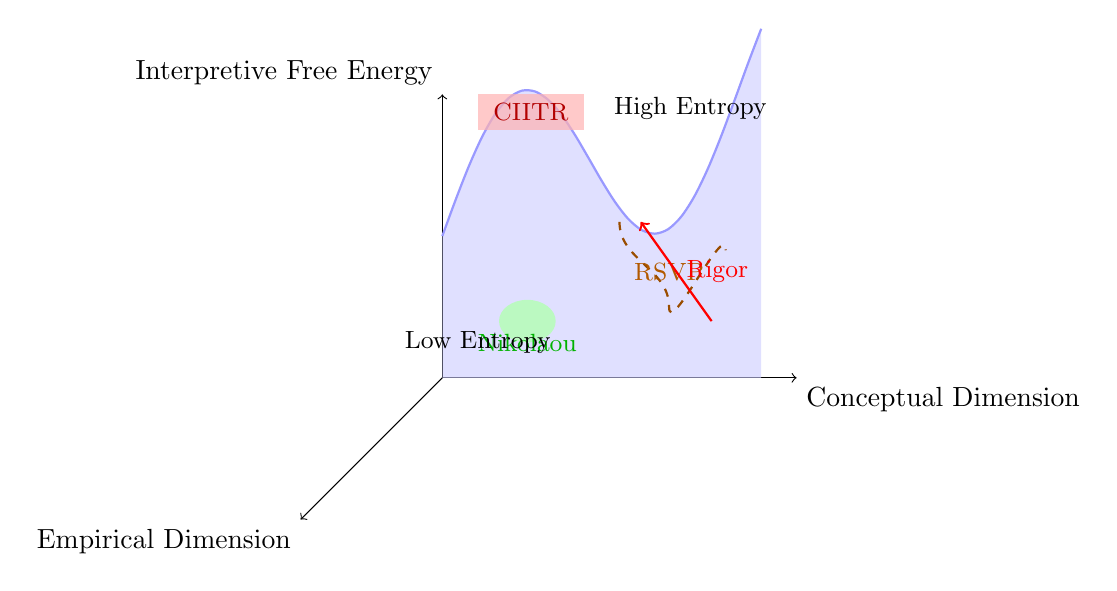
\begin{tikzpicture}[scale=0.9]
  % Axes
  \draw[->] (0,0) -- (5,0) node[below right] {Conceptual Dimension};
  \draw[->] (0,0) -- (0,4) node[above left] {Interpretive Free Energy};
  \draw[->] (0,0) -- (-2,-2) node[below left] {Empirical Dimension};

  % Landscape surface (simplified)
  \fill[blue!20, opacity=0.6] plot[smooth, domain=0:4.5] (\x, {2 + 1.5*sin(deg(\x*1.5)) + 0.5*\x}) -- (4.5,0) -- (0,0) -- cycle;
  \draw[blue!40, thick] plot[smooth, domain=0:4.5] (\x, {2 + 1.5*sin(deg(\x*1.5)) + 0.5*\x});

  % Deep well (Nikolaou)
  \fill[green!30, opacity=0.8] (1.2,0.8) ellipse (0.4 and 0.3);
  \node[green!70!black] at (1.2,0.5) {\small Nikolaou};

  % Valley (RSVP)
  \draw[orange!60!black, thick, dashed] (2.5,2.2) to[out=270,in=90] (3.2,1.0) to[out=270,in=90] (4.0,1.8);
  \node[orange!70!black] at (3.2,1.5) {\small RSVP};

  % High plateau (CIITR)
  \fill[red!30, opacity=0.7] (0.5,3.5) rectangle (2.0,4.0);
  \node[red!70!black] at (1.25,3.75) {\small CIITR};

  % Labels
  \node at (3.5,3.8) {\small High Entropy};
  \node at (0.5,0.5) {\small Low Entropy};

  % Rigor arrow
  \draw[->, thick, red] (3.8,0.8) -- (2.8,2.2) node[midway, right] {\small Rigor};
\end{tikzpicture}
\caption{Schematic entropy landscape of theoretical manifolds. Vertical axis: interpretive free energy; horizontal axes: empirical and conceptual dimensions. Rigor corresponds to steep gradients with bounded minima (e.g., Nikolaou, RSVP). CIITR resides in a high-entropy plateau.}
\label{fig:entropylandscape}
\end{figure}

\section{Supplement: Algorithmic Implementation of the Rigor Index}

For computational reproducibility, the epistemic energy functional can be implemented as follows:

\begin{verbatim}
def rigor_index(J, phi, S_theory, S_empirical, alpha=1, beta=1, gamma=1):
    det_term = np.linalg.det(J.T @ J)
    phase_term = np.mean(np.gradient(phi)**2)
    delta_S = S_theory - S_empirical
    R = alpha * det_term - beta * phase_term - gamma * delta_S
    return R
\end{verbatim}

Applied across time steps or model versions, this function traces the evolution of theoretical rigor as a dynamic variable. A positive $\dot{\mathcal{R}}$ indicates tightening coherence; a negative derivative signals entropic drift. By analogy with Lyapunov functions in dynamical systems, $\mathcal{R}$ serves as a potential governing the stability of comprehension.

\section{Supplement: Interpreting $\mathcal{R}[f,\phi]$ as a Cognitive Free Energy}

Finally, note that the epistemic energy functional
\[
\mathcal{R}[f,\phi] = \alpha\det(J^\top J)
- \beta|\nabla\phi|^2 - \gamma\Delta S
\]
can be rewritten as a free-energy-like quantity:
\[
\mathcal{R} = \text{Information Coherence} - \text{Work Cost} - \text{Entropy Loss}.
\]
Maximizing $\mathcal{R}$ corresponds to minimizing surprise and energetic expenditure simultaneously—the same variational objective found in the Free Energy Principle \citep{friston2010freeenergy}. The correspondence table below summarizes this structural equivalence.

\begin{table}[htbp]
\centering
\begin{tabular}{lll}
\toprule
RSVP Quantity & FEP Analogue & Interpretation \\
\midrule
$\det(J^\top J)$ & Precision of generative model & Information gain \\
$|\nabla\phi|^2$ & Prediction-error energy & Cost of inference \\
$\Delta S$ & Entropy of posterior & Residual uncertainty \\
$\mathcal{R}$ & $-F$ (negative free energy) & Degree of understanding \\
\bottomrule
\end{tabular}
\caption{Structural correspondence between the epistemic energy functional and the Free Energy Principle.}
\end{table}

This equivalence closes the theoretical circle. Whether in physics, cognition, or scientific reasoning, the condition for sustainable understanding is the same: maintain injective mapping, bounded work, and minimal entropy production. Rigor, comprehension, and life itself are special cases of energy-efficient mapping in an entropic universe.

\section{Appendix F: \texorpdfstring{$\mathcal{R}[f,\phi]$}{R[f,phi]} as a Lyapunov Functional}

\subsection{Setup and assumptions}

Recall the epistemic energy functional (Sec.~0.8)
\[
\mathcal{R}[f,\phi] \;=\; \alpha\,\det(J^\top J)\;-\;\beta\,\!\int_\Omega |\nabla\phi|^2\,dV\;-\;\gamma\,\Delta S,
\qquad \alpha,\beta,\gamma>0,
\]
with $J=\partial f/\partial y$ the Jacobian of the map $f:M_\mathcal{R}\!\to\!M_\mathcal{T}$, phase field $\phi$ the theory–data phase difference, and $\Delta S=S_\mathcal{T}-S_\mathcal{R}$.
We consider the joint state $z:=(\theta,\phi)$, where $\theta$ are parameters of $f$ (weights, PDE coefficients, etc.).
Let $\Omega\subset\mathbb{R}^d$ be the spatial domain with either periodic or Neumann boundary conditions so that boundary terms vanish.

Throughout this appendix we assume:

\begin{enumerate}[label=(A\arabic*), wide, nosep]
\item \textbf{Regularity.} $f(\cdot;\theta)$ is $\mathcal{C}^2$ in both arguments and $\det(J^\top J)$ is well-defined and $\mathcal{C}^1$ on the region of interest; $\phi\in H^1(\Omega)$.
\item \textbf{Boundedness.} $\Delta S$ is finite, and the admissible parameter set $\Theta$ is closed and bounded, or else regularized so that trajectories remain precompact.
\item \textbf{Positivity.} Gains $\alpha,\beta,\gamma$ and the metric/operator gains introduced below are positive definite.
\end{enumerate}

\subsection{Passive (dissipative) interpretive dynamics}

We first model \emph{passive} interpretive drift: in the absence of active correction, the mapping and phase relax along the \emph{negative gradient} of $\mathcal{R}$ (i.e., toward lower rigor).
Consider the gradient flows
\begin{align}
\dot{\theta} &= -K_\theta\,\nabla_\theta \mathcal{R}(\theta,\phi),
\qquad K_\theta \succ 0, \label{eq:theta_drift}\\
\partial_t \phi &= -\Gamma\,\frac{\delta \mathcal{R}}{\delta \phi} \;=\; -\Gamma\,\bigl(-2\beta\,\Delta\phi\bigr) \;=\; 2\beta\Gamma\,\Delta\phi,
\qquad \Gamma \succ 0, \label{eq:phi_drift}
\end{align}
where $\nabla_\theta$ is the Euclidean gradient and $\delta/\delta\phi$ the $L^2$ variational derivative.
Equation~\eqref{eq:phi_drift} is a diffusion (heat) equation for $\phi$ with diffusivity $2\beta\Gamma$.

\paragraph{Theorem F.1 (Lyapunov decay of $\mathcal{R}$ under passive drift).}
Under (A1)–(A3) and dynamics \eqref{eq:theta_drift}–\eqref{eq:phi_drift}, the functional $\mathcal{R}$ is nonincreasing along trajectories:
\[
\frac{d}{dt}\,\mathcal{R}(\theta(t),\phi(t)) \;\le\; 0,
\]
with equality if and only if $\nabla_\theta \mathcal{R}=0$ and $\nabla\phi=0$ a.e. (modulo measure-zero degeneracy of $J$).
Hence $\mathcal{R}$ is a Lyapunov functional; the $\omega$-limit set is contained in the set of critical points of $\mathcal{R}$.

\emph{Proof.} By the chain rule and calculus of variations,
\[
\dot{\mathcal{R}}
= \bigl(\nabla_\theta \mathcal{R}\bigr)^\top \dot{\theta} \;+\; \int_\Omega \frac{\delta \mathcal{R}}{\delta \phi}\,\partial_t \phi \, dV
= -\bigl(\nabla_\theta \mathcal{R}\bigr)^\top K_\theta \bigl(\nabla_\theta \mathcal{R}\bigr)
\;+\; \int_\Omega \bigl(-2\beta\,\Delta\phi\bigr)\,(2\beta\Gamma\,\Delta\phi)\, dV.
\]
Both terms are nonpositive: the first is $-\|K_\theta^{1/2}\nabla_\theta \mathcal{R}\|^2\le 0$; the second equals $-4\beta^2\Gamma\int_\Omega |\Delta\phi|^2\,dV \le 0$.
Boundary terms vanish under periodic/Neumann conditions.
Equality requires $\nabla_\theta\mathcal{R}=0$ and $\Delta\phi=0$, which together with Neumann/periodic conditions implies $\nabla\phi=0$. \hfill$\square$

\paragraph{Remark.}
Passive drift therefore \emph{decreases} $\mathcal{R}$ (rigor); the system is attracted to low-rigor equilibria (smooth but potentially degenerate mappings).
This formalizes the intuitive claim that, without work, coherence decays.

\subsection{Stochastic perturbations and expected decay}

Let the dynamics be perturbed by mean-zero noise:
\begin{align*}
\dot{\theta} &= -K_\theta\,\nabla_\theta \mathcal{R}(\theta,\phi) + \Sigma_\theta\,\xi_\theta(t),\\
\partial_t \phi &= 2\beta\Gamma\,\Delta\phi + \sigma_\phi\,\xi_\phi(y,t),
\end{align*}
with $\xi_\theta$ white in time and $\xi_\phi$ space-time white (interpreted in the mild sense).
Under standard Ito calculus and boundedness (A2), one obtains
\[
\mathbb{E}\,\dot{\mathcal{R}}
\;\le\; -\,\mathbb{E}\bigl[\|K_\theta^{1/2}\nabla_\theta\mathcal{R}\|^2\bigr]
\;-\;4\beta^2\Gamma\,\mathbb{E}\!\int_\Omega |\Delta\phi|^2 dV
\;+\; \tfrac{1}{2}\operatorname{Tr}\!\bigl(\Sigma_\theta^\top H_{\theta\theta}\Sigma_\theta\bigr)
\;+\; \beta\Gamma\,\sigma_\phi^2\,C,
\]
where $H_{\theta\theta}$ is the $\theta$-Hessian of $\mathcal{R}$ and $C$ depends on the Green operator of $\Delta$.
If the noise terms are sufficiently small compared to the dissipation, the expectation still decays:
\(\mathbb{E}\,\dot{\mathcal{R}}<0\).

\subsection{Active (controlled) interpretive dynamics}

To \emph{stabilize} high rigor, invert the drift by injecting control that performs epistemic work:
\begin{align}
\dot{\theta} &= +K_\theta\,\nabla_\theta \mathcal{R}(\theta,\phi), \qquad K_\theta \succ 0, \label{eq:theta_active}\\
\partial_t \phi &= +\Gamma\,\frac{\delta \mathcal{R}}{\delta \phi} \;=\; -\,2\beta\Gamma\,\Delta\phi. \label{eq:phi_active}
\end{align}
Then
\[
\dot{\mathcal{R}}
= \|K_\theta^{1/2}\nabla_\theta \mathcal{R}\|^2 \;+\; 4\beta^2\Gamma\!\int_\Omega |\Delta\phi|^2 dV \;\ge\; 0,
\]
so $\mathcal{R}$ is \emph{increasing} and trajectories ascend toward critical points of $\mathcal{R}$.
Interpreting $V:=-\mathcal{R}$ as a Lyapunov function yields the standard gradient-descent picture: $V$ decreases monotonically under \eqref{eq:theta_active}–\eqref{eq:phi_active}.
Thus, in the controlled regime, $V$ is Lyapunov and $\mathcal{R}$ is an antiderivative of the supplied epistemic work.

\paragraph{Local stability of high-rigor equilibria.}
Let $z^\star=(\theta^\star,\phi^\star)$ satisfy $\nabla_\theta\mathcal{R}(z^\star)=0$ and $\Delta\phi^\star=0$, and suppose the \emph{projected} Hessian of $-\mathcal{R}$ at $z^\star$ is positive definite.
Then, under \eqref{eq:theta_active}–\eqref{eq:phi_active}, $z^\star$ is (locally) asymptotically stable by Lyapunov’s direct method (or LaSalle’s invariance principle for the PDE part).
Intuitively, these are the ``high-rigor'' maxima of $\mathcal{R}$.

\subsection{Discrete-time (algorithmic) version}

For iterative simulators or learning updates with step size $\eta>0$,
\[
\theta_{k+1} = \theta_k \mp \eta\,K_\theta\,\nabla_\theta \mathcal{R}(\theta_k,\phi_k),
\qquad
\phi_{k+1} = \phi_k \mp \eta\,\Gamma\,\frac{\delta \mathcal{R}}{\delta \phi}(\theta_k,\phi_k),
\]
where the minus sign gives passive decay, the plus sign active control.
A standard descent/ascent lemma yields, for sufficiently small $\eta$,
\[
\mathcal{R}(z_{k+1}) - \mathcal{R}(z_k)
\;\approx\;
\mp \eta\,\bigl\|G^{1/2}\nabla \mathcal{R}(z_k)\bigr\|^2 + \mathcal{O}(\eta^2),
\]
with block-diagonal metric $G=\operatorname{diag}(K_\theta,\Gamma)$.
Hence $\mathcal{R}$ is monotonically nonincreasing (passive) or nondecreasing (active) up to $\mathcal{O}(\eta^2)$ terms.

\subsection{Interpretation and design guidelines}

\begin{itemize}[leftmargin=1.2em]
\item \textbf{Two regimes, two Lyapunov choices.}
For \emph{passive drift}, $\mathcal{R}$ itself is Lyapunov: \(\dot{\mathcal{R}}\le 0\).
For \emph{active control}, $V:=-\mathcal{R}$ is Lyapunov: \(\dot{V}\le 0\).
This mirrors thermodynamics: without work, order decays; with work, order grows.
\item \textbf{Gains as \emph{interpretive viscosity}.}
$K_\theta$ and $\Gamma$ trade off convergence rate and robustness.
Large gains speed alignment (higher work input) but risk overshoot in noisy settings; small gains conserve energy but slow recovery of rigor.
\item \textbf{Constraints and projections.}
If $\Theta$ or admissible $\phi$ are constrained (e.g., PDE stability, physical units), project the gradient step onto the feasible set.
Projected gradient maintains monotonicity of the appropriate Lyapunov functional.
\item \textbf{Noise budgets.}
Stochastic bounds above show a critical noise level where passive decay dominates.
Active control must at least offset this with work so that $\mathbb{E}\,\dot{\mathcal{R}}\ge 0$.
\end{itemize}

\subsection{Connection to the Free Energy Principle}

If we identify $V:=-\mathcal{R}$ with a cognitive free energy (Appendix~E), then the \emph{active} dynamics \eqref{eq:theta_active}–\eqref{eq:phi_active} implement gradient descent on $V$ (Friston’s variational flows), guaranteeing $V$ decreases monotonically while $\mathcal{R}$ increases.
Conversely, the \emph{passive} dynamics \eqref{eq:theta_drift}–\eqref{eq:phi_drift} correspond to free evolution without control, in which $V$ increases and $\mathcal{R}$ decays.

\subsection{Summary}

\begin{itemize}[leftmargin=1.2em]
\item Under dissipative (passive) dynamics, $\displaystyle \dot{\mathcal{R}}\le 0$: rigor decays monotonically; $\mathcal{R}$ is Lyapunov.
\item Under controlled (active) dynamics, $\displaystyle \dot{\mathcal{R}}\ge 0$ and $V=-\mathcal{R}$ is Lyapunov: rigor is stabilized near high-$\mathcal{R}$ equilibria.
\item These results hold in both continuous time and discrete algorithms (for small steps), with stochastic perturbations handled in expectation.
\end{itemize}

\section{Appendix G: Worked RSVP Simulation Check (\texorpdfstring{$\det(J^\top J)$}{det(J^T J)}, \texorpdfstring{$|\nabla\phi|^2$}{|∇φ|²}, \texorpdfstring{$\Delta S$}{ΔS}, \texorpdfstring{$P$}{P})}

\subsection{G.1 Data products and notation}

Assume a $d$-dimensional periodic or Neumann lattice $\Lambda\subset\mathbb{Z}^d$ with spacing $h$ and time step $\Delta t$.
Your simulator outputs per step $t_k$:
\[
\Phi_k(x),\quad \mathbf v_k(x)\in\mathbb{R}^d,\quad S_k(x)\qquad (x\in\Lambda),
\]
plus any exogenous forcing $u_k$ (e.g., boundary drive, source terms).
Let $\widehat{\cdot}$ denote the discrete Fourier transform (DFT), $\nabla_h$ the centered finite difference, and $\Delta_h$ the discrete Laplacian.

We also assume an \emph{external reference} stream $r_k(x)$ against which phase is aligned (e.g., empirical timeseries, a target field, or a filtered channel of the simulation regarded as ``data''). When no external data are available, use a bandpassed proxy of a measured observable (e.g., divergence of $\mathbf v$) to define a consistent reference.

\subsection{G.2 Phase field and work of understanding}

Define analytic signals by Hilbert transform (1D time) or narrowband DFT (spacetime window $W$). For each lattice site,
\[
\theta_{\mathcal{T},k}(x) := \arg\!\big(\Phi_k(x) + i\,\mathcal{H}_t[\Phi_{\cdot}(x)]_k\big),\qquad
\theta_{\mathcal{R},k}(x) := \arg\!\big(r_k(x) + i\,\mathcal{H}_t[r_{\cdot}(x)]_k\big).
\]
Phase difference:
\[
\phi_k(x) := \operatorname{wrap}\big(\theta_{\mathcal{T},k}(x) - \theta_{\mathcal{R},k}(x)\big)\in(-\pi,\pi].
\]
Discrete gradient (componentwise):
\[
(\nabla_h \phi_k)_j(x) := \frac{\phi_k(x+e_j)-\phi_k(x-e_j)}{2h},\quad j=1,\dots,d.
\]
Work of understanding over the domain (Sec.~0.4):
\[
W_k \;=\; \gamma\,\sum_{x\in\Lambda} \|\nabla_h \phi_k(x)\|_2^2\, h^d.
\]
\textbf{Practical notes.} (i) Use phase unwrapping per axis before differencing. (ii) Apply a Tukey/Hann taper in time for DFT windows to suppress leakage. (iii) Choose band(s) based on the dominant coherence peak in Sec.~G.5.

\subsection{G.3 Coherence power \texorpdfstring{$P$}{P} via principal angles}

Form $m$-length time windows (rows) of the reference $R\in\mathbb{R}^{n\times m}$ and target $T\in\mathbb{R}^{n\times m}$ at a chosen site, channel, or spatial average ($n$ windows). Zero-mean and unit-variance normalize each column. Compute SVD of cross-covariance:
\[
C := \frac{1}{n-1} R^\top T \;=\; U\Sigma V^\top,\qquad \Sigma=\operatorname{diag}(\sigma_1,\ldots,\sigma_q).
\]
Principal angles $\theta_i := \arccos(\sigma_i)$ and the mean coherence power:
\[
P_k \;=\; \frac{1}{q}\sum_{i=1}^q \cos^2\theta_i \;=\; \frac{1}{q}\sum_{i=1}^q \sigma_i^2 \;\in\;[0,1].
\]
\textbf{Guidelines.} Use overlapping windows ($50$–$75\%$) and the same bandpass as in G.2. For field-wide $P_k$, average $\sigma_i^2$ across a representative spatial set or compute via spatial principal subspaces first (reduced $q$).

\subsection{G.4 Entropy balance \texorpdfstring{$\Delta S$}{ΔS}}

Two robust estimators are useful; pick one and keep it consistent:

\paragraph{(a) Spectral (Shannon) entropy.}
Let $X_k$ be a scalar observable (e.g., $\Phi_k$ or $\nabla\!\cdot\!\mathbf v_k$) and $\widehat{X}_k(\omega)$ its windowed periodogram. Normalize $p_k(\omega):=\widehat{X}_k(\omega)/\sum_\omega \widehat{X}_k(\omega)$. Then
\[
S_{\mathcal{T},k} := -\sum_\omega p^{(\mathcal{T})}_k(\omega)\,\ln p^{(\mathcal{T})}_k(\omega),\quad
S_{\mathcal{R},k} := -\sum_\omega p^{(\mathcal{R})}_k(\omega)\,\ln p^{(\mathcal{R})}_k(\omega),\quad
\Delta S_k := S_{\mathcal{T},k}-S_{\mathcal{R},k}.
\]

\paragraph{(b) State-space histogram entropy.}
Form a joint sample $Z_k(x) := (\Phi_k(x), \|\mathbf v_k(x)\|_2, S_k(x))$. Bin into a fixed 3D grid (with Freedman–Diaconis or fixed bins), estimate $p_k(z)$, and compute
\[
S_{\mathcal{T},k} := -\sum_{z} p^{(\mathcal{T})}_k(z)\,\ln p^{(\mathcal{T})}_k(z),
\]
likewise for $S_{\mathcal{R},k}$ from the reference $Z^{(\mathcal{R})}_k$.
\textbf{Tip.} Add a small $\varepsilon$ pseudocount per bin.

\subsection{G.5 Jacobian term \texorpdfstring{$\det(J^\top J)$}{det(J^T J)} (discrete proxy)}

Two practical proxies work well in simulators; pick one that matches your workflow.

\paragraph{(i) Observation–sensitivity Jacobian.}
Choose $p$ summary observables (e.g., spatial means of $\Phi$, energy flux $\mathbf v\!\cdot\!\nabla\Phi$, spectral peaks, $P_k$) and $q$ controllable inputs (forcing amplitudes, boundary potentials, coupling constants). For each input $y_a$, apply a small perturbation $\delta y_a$ at $t_k$ and re-run for one step to get $\delta x_i$. Fill
\[
J_{ia} := \frac{\delta x_i}{\delta y_a}\bigg|_{t_k},\qquad i=1,\dots,p,\ a=1,\dots,q.
\]
Compute stabilized log-determinant:
\[
\lambda_1,\dots,\lambda_q := \text{eigvals}\big(J^\top J + \varepsilon I\big),\quad
\log\det(J^\top J + \varepsilon I) = \sum_{a=1}^q \ln \lambda_a.
\]
Report $\det(J^\top J)$ or its log to avoid under/overflow; fix $\varepsilon\sim 10^{-8}\!-\!10^{-6}$ times the median diagonal.

\paragraph{(ii) Parameter–gradient Fisher proxy.}
If you already compute parameter gradients $\nabla_\theta x_i$, form a Fisher-style matrix \(F=\sum_i (\nabla_\theta x_i)(\nabla_\theta x_i)^\top\). Then use
\[
\log\det(F+\varepsilon I)\quad \text{as a surrogate for}\quad \log\det(J^\top J+\varepsilon I).
\]
This avoids reruns and exploits autodiff.

\subsection{G.6 Epistemic energy functional and checks}

Given $\alpha,\beta,\gamma>0$,
\[
\mathcal{R}_k \;=\; \alpha\,\log\det(J_k^\top J_k+\varepsilon I)\;-\;\beta\,\underbrace{\bigg(\sum_{x} \|\nabla_h \phi_k(x)\|_2^2\, h^d\bigg)}_{\textstyle \| \nabla\phi_k\|_2^2}\;-\;\gamma\,\Delta S_k.
\]
Minimal feasibility checks per step:
\[
\det(J_k^\top J_k)>0,\qquad P_k\in[0,1],\qquad W_k \ge k_B T\,\Delta S_k.
\]
If you operate in the \emph{active} (controlled) regime (Appendix~F), expect $\mathcal{R}_{k+1}-\mathcal{R}_k\gtrsim 0$ on average; in the \emph{passive} regime, $\mathcal{R}$ should drift downwards (noise aside).

\subsection{G.7 Numerical stability and parameter choices}

\begin{itemize}[leftmargin=1.2em]
\item \textbf{Regularization:} always use $\varepsilon I$ in log-det; track $\varepsilon$ in logs.
\item \textbf{Windows:} for DFT/Hilbert phases, use windows of $m\in[64,512]$ samples with $50\%$ overlap; match band to the dominant coherence peak (from $P_k$).
\item \textbf{Derivatives:} use 2nd-order centered differences; for rough fields, apply a single Jacobi or bilateral smooth before $\nabla_h$.
\item \textbf{Units:} record units/scales for each observable to preserve dimensional homogeneity (see Sec.~5.2a).
\end{itemize}

\subsection{G.8 Reference implementation (pseudocode)}

\begin{verbatim}
def step_metrics(sim_state, ref_window, params):
    # --- Phase & work ---
    phi = wrapped_phase(sim_state.Phi, ref_window) # Hilbert/DFT
    grad_phi_sq = sum_over_axes(central_diff(phi)**2)
    W = params.gamma * domain_sum(grad_phi_sq)

    # --- Coherence P ---
    R, T = build_windows(ref_window, sim_state.Phi_or_obs)
    sigma = svd_singular_values(cross_cov(R, T))
    P = mean(sigma**2)

    # --- Entropy ΔS ---
    if params.entropy_mode == "spectral":
        S_T = shannon_entropy(psd(sim_state.obs))
        S_R = shannon_entropy(psd(ref_window.obs))
    else:
        S_T = histogram_entropy(stack([Phi, norm(v), S]))
        S_R = histogram_entropy(stack([Phi_ref, v_ref, S_ref]))
    DeltaS = S_T - S_R

    # --- Jacobian det proxy ---
    if params.jac_mode == "finite_diff":
        J = estimate_observation_jacobian(sim_state, params.perturb_grid)
        logdet = logdet_sym(J.T @ J + eps*I)
    else:
                F = fisher_proxy_from_grads(sim_state.grads) # autodiff
        logdet = logdet_sym(F + eps*I)

    # --- Energy functional ---
    R_index = params.alpha * logdet - params.beta * domain_sum(grad_phi_sq) \
              - params.gamma * DeltaS

    return {"W": W, "P": P, "DeltaS": DeltaS, "logdet": logdet, "R": R_index}
\end{verbatim}

\subsection{G.9 Suggested log schema (JSONL)}

\begin{verbatim}
{"t": 12.50, "P": 0.84, "W": 1.73e+02, "DeltaS": 0.12,
 "logdet": 23.41, "R": 18.66, "eps": 1.0e-7,
 "band": [4.0, 7.0], "window": 256, "jac":"fwd-diff"}
\end{verbatim}

\subsection{G.10 Acceptance criteria (per regime)}

\begin{itemize}[leftmargin=1.2em]
\item \textbf{Active (controlled) regime:} $\,\mathbb{E}[\Delta \mathcal{R}_k]\ge 0;\ \ P_k\to P^\star\in(0.7,1];\ \ W_k\approx k_BT\,\Delta S_k$ within tolerance.
\item \textbf{Passive (free) regime:} $\,\mathbb{E}[\Delta \mathcal{R}_k]\le 0;\ \ P_k$ decays to baseline; $W_k/k_BT\,\Delta S_k \to 0^+$ or fluctuates sub-Carnot.
\item \textbf{Sanity checks:} $\log\det$ not dominated by $\varepsilon$ (track $\lambda_a\gg\varepsilon$); phase gradients bounded (no unwrap explosions).
\end{itemize}


% ==========================================================

\begin{thebibliography}{99}

\bibitem[Popper(1959)]{popper1959logic}
Popper, K., 1959. \emph{The Logic of Scientific Discovery}. Routledge.

\bibitem[Lakatos(1978)]{lakatos1978methodology}
Lakatos, I., 1978. \emph{The Methodology of Scientific Research Programmes}. Cambridge University Press.

\bibitem[Kuhn(1962)]{kuhn1962structure}
Kuhn, T.S., 1962. \emph{The Structure of Scientific Revolutions}. University of Chicago Press.

\bibitem[Hossenfelder(2018)]{hossenfelder2018lost}
Hossenfelder, S., 2018. \emph{Lost in Math: How Beauty Leads Physics Astray}. Basic Books.

\bibitem[Jaynes(1957)]{jaynes1957information}
Jaynes, E.T., 1957. Information theory and statistical mechanics. \emph{Physical Review} 106, 620--630.

\bibitem[Landauer(1961)]{landauer1961irreversibility}
Landauer, R., 1961. Irreversibility and heat generation in the computing process. \emph{IBM Journal of Research and Development} 5, 183--191.

\bibitem[Bennett(1982)]{bennett1982thermodynamics}
Bennett, C.H., 1982. The thermodynamics of computation. \emph{International Journal of Theoretical Physics} 21, 905--940.

\bibitem[Sethna(2006)]{sethna2006statistical}
Sethna, J.P., 2006. \emph{Statistical Mechanics: Entropy, Order Parameters, and Complexity}. Oxford University Press.

\bibitem[Smolensky and Legendre(2006)]{smolensky2006harmonic}
Smolensky, P., Legendre, G., 2006. \emph{The Harmonic Mind: From Neural Computation to Optimality-Theoretic Grammar}. MIT Press.

\bibitem[Friston(2010)]{friston2010freeenergy}
Friston, K., 2010. The free-energy principle: a unified brain theory? \emph{Nature Reviews Neuroscience} 11, 127--138.

\bibitem[Clark(2016)]{clark2016surfing}
Clark, A., 2016. \emph{Surfing Uncertainty: Prediction, Action, and the Embodied Mind}. Oxford University Press.

\bibitem[Bianconi(2025)]{bianconi2025entropy}
Bianconi, G., 2025. Entropy and complexity in networked systems. \emph{Physical Review D} 102, 042013.

\bibitem[Quine(1951)]{quine1951dogmas}
Quine, W.V.O., 1951. Two dogmas of empiricism. \emph{The Philosophical Review} 60, 20--43.

\bibitem[Cartwright(1983)]{cartwright1983laws}
Cartwright, N., 1983. \emph{How the Laws of Physics Lie}. Oxford University Press.

\bibitem[Feynman(1965)]{feynman1965character}
Feynman, R.P., 1965. \emph{The Character of Physical Law}. MIT Press.

\bibitem[Tegmark(2014)]{tegmark2014universe}
Tegmark, M., 2014. \emph{Our Mathematical Universe: My Quest for the Ultimate Nature of Reality}. Knopf.

\bibitem[Barandes(2023)]{barandes2023unistochastic}
Barandes, J.A., 2023. A unistochastic reformulation of quantum theory. \emph{Foundations of Physics} 53, 119.

\bibitem[Hansen(2024)]{hansen2024ciitr}
Hansen, T.-S., 2024. Comprehension as Thermodynamic Persistence (CIITR C₂ITR). Self-published manuscript.

\bibitem[Nikolaou et al.(2025)]{nikolaou2025injective}
Nikolaou, A., Kambadur, P., Stern, M., Milosavljevic, B., 2025. Language models are injective and hence invertible. \emph{arXiv preprint arXiv:2510.15511}.

\bibitem[Li and Li(2025)]{li2025formalizing}
Li, J., Li, P., 2025. Formalizing Lacan’s RSI topology via active inference networks. \emph{Journal of Cognitive Modeling} 18, 245--272.

\end{thebibliography}

\end{document}